%% packages
\documentclass{article}
\usepackage[a4paper, left=2.0cm, right=2.0cm, top=3.5cm]{geometry}
\usepackage[ngerman]{babel}
\usepackage{graphicx}
\usepackage{multicol}
\usepackage{amssymb}
\usepackage{titlesec}
\usepackage{wrapfig}
\usepackage{blindtext}
\usepackage{lipsum}
\usepackage{caption}
\usepackage{listings}
\usepackage{fancyhdr}
\usepackage{nopageno}
\usepackage{authblk}
\usepackage{amsmath} % tons of math stuff
\usepackage{mathtools} % e.g. alignment within matrix
%\usepackage{bm} % provides shorthand for bold in math mode
\usepackage{dsfont} % \mathds makes double stroke digits
\usepackage{esdiff} % provides \diff
%\usepackage[ISO]{diffcoeff}
\usepackage{xcolor}
\usepackage{csquotes} % e.g. provides \enquote
\usepackage[separate-uncertainty=true]{siunitx} % units
\usepackage{xcolor} % colored text
\usepackage{csvsimple}
\usepackage{subcaption}
\usepackage{physics}
\usepackage{hyperref}
\usepackage{nameref}
\hypersetup{colorlinks=true, linkcolor=black, pdfhighlight={/N}}
\usepackage{tcolorbox}
\usepackage{amsthm}
\usepackage{float}
\usepackage{enumitem}




%\fancyhf[]{}

%% custom stuff
% own units
\DeclareSIUnit \VSS {\ensuremath{V_\mathrm{SS}}}
\DeclareSIUnit \VS {\ensuremath{V_\mathrm{S}}}
\DeclareSIUnit \Veff {\ensuremath{V_\mathrm{eff}}}
\DeclareSIUnit \Vpp {\ensuremath{V_\mathrm{pp}}}
\DeclareSIUnit \Vp {\ensuremath{V_\mathrm{p}}}
\DeclareSIUnit \VRMS {\ensuremath{V_\mathrm{RMS}}}
\DeclareSIUnit \ASS {\ensuremath{A_\mathrm{SS}}}
\DeclareSIUnit \AS {\ensuremath{A_\mathrm{S}}}
\DeclareSIUnit \Aeff {\ensuremath{A_\mathrm{eff}}}
\DeclareSIUnit \App {\ensuremath{A_\mathrm{pp}}}
\DeclareSIUnit \Ap {\ensuremath{A_\mathrm{p}}}
\DeclareSIUnit \ARMS {\ensuremath{A_\mathrm{RMS}}}

% change subsection numbering to capital letters
\newcommand{\subsectionAlph}{ \renewcommand{\thesubsection}{\arabic{section}.\Alph{subsection}} }
% change subsection numbering to lowercase letters
\newcommand{\subsectionalph}{ \renewcommand{\thesubsection}{\arabic{section}.\alph{subsection}} }
% change subsubsection numbering to lowercase letters
\newcommand{\subsubsectionalph}{ \renewcommand{\thesubsubsection}{\arabic{section}.\arabic{subsection}.\alph{subsubsection}} }
% own fig. that works with multicols
\newenvironment{Figure}
  {\par\medskip\noindent\minipage{\linewidth}}
  {\endminipage\par\medskip}
\newcommand*{\inputPath}{./plot} % prepend this command to the argument of all input commands
\graphicspath{ {./images/}{./figure/} }
% own enviroment for definitions
\newenvironment{definition}[1]
{\begin{quote} \noindent \textbf{\textit{#1\ifx&#1& \else : \fi}} \itshape}
{\end{quote}}


% own commands
% \newcommand{\rarr}{$\to\,$} %A$\,\to\,$B
\newcommand{\defc}{black}
\newcommand{\colorT}[2][blue]{\color{#1}{#2}\color{\defc}}
\newcommand{\redq}{\color{red}(?)\color{\defc}}
\newcommand{\question}[1]{\colorT[purple]{\textbf{(#1)}}}
\newcommand{\todo}[1]{\colorT[red]{\textbf{(#1)}}}
\newcommand{\mr}{\mathrm}

%% preparation
\begin{titlepage}
  \title{Praktikum Atome, Moleküle, kondensierte Materie \\ Versuch 401: Elektronische Übergänge in Atomen}
  \author[1]{Carlos Pascua\thanks{s87cpasc@uni-bonn.de}}
  \author[1]{Michael Vogt\thanks{s65mvogt@uni-bonn.de}}
  \affil[1]{Uni Bonn}
  %\date{\today}
\end{titlepage}


%% document
\begin{document}

\pagenumbering{gobble}
\maketitle
\tableofcontents
\newpage
\pagenumbering{arabic}

\pagestyle{fancy}
\fancyhead[R]{\thepage}
\fancyhead[L]{\leftmark}

\begin{multicols}{2}

\section*{Einleitung}
In diesem Versuch wird die Energieaufspaltung von Energie-Niveaus in Cadmium durch den Zeeman-Effekt untersucht.
Daraus wird das Bohrsche Magneton bestimmt sowie Eigenschaften des verwendeten Fabry-Perot-Etalons errechnet.

Anschließend wird das Franck-Hertz-Experiment durchgeführt, um die Energiedifferenz zwischen dem 6S- und 6P-Zustand von Quecksilber zu bestimmen.


\section{Zeeman-Effekt}
Im ersten Versuchsteil wird anhand einer Cadmiumlampe in einem Magnetfeld der Zeeman-Effekt auf die Zustände $^1D_2$ und $^1P_1$ untersucht.
Der verwendete Aufbau ist in Abb. \ref{fig:zeeman-aufbau} zu sehen.
\begin{figure}[H]
  \centering
  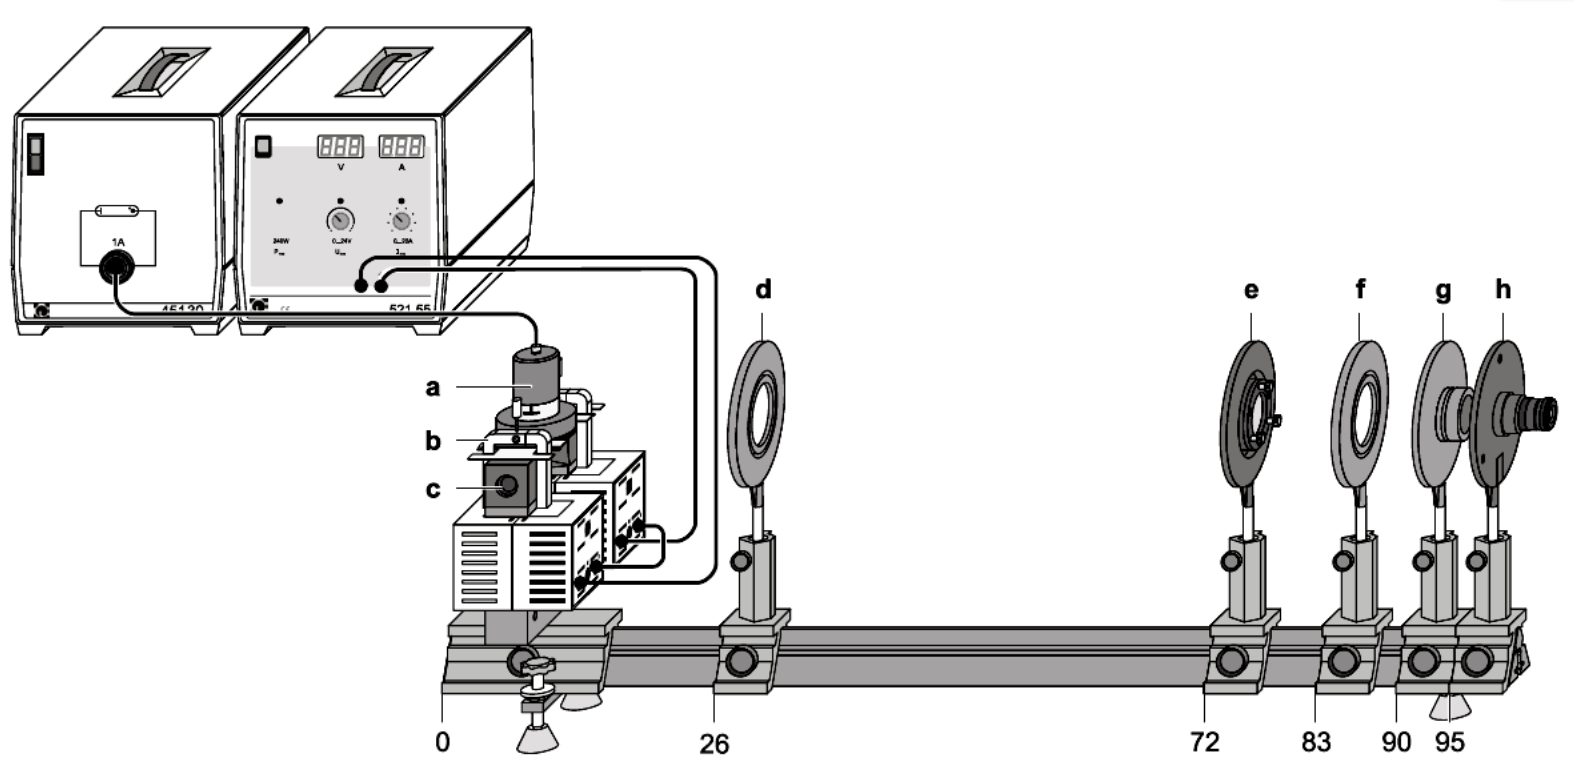
\includegraphics[width=\linewidth]{zeeman-aufbau}
  \caption{Versuchsaufbau Zeeman-Effekt \cite{Leybold}}
  \label{fig:zeeman-aufbau}
\end{figure}
% Der $^1D_2$-Zustand hat Aufspaltungen in $M_J = -2,\,\dots\,,2$ und $^1P_1$ in $M_J=-1,0,1$.
% Es kann also Übergänge mit $\Delta M_J = -1, 0, 1$ geben.
% In Abhängigkeit des $\Delta M$-Werts gibt es verschiedene
Folgende wichtige Bestandteile sind zu sehen \cite{Anleitung}:
\begin{enumerate}[label=\alph*.]
  \item Cadmium-Lampe
  \item Klammern
  \item Polschuhe
  \item Kondensorlinse
  \item Polarisationsfilter
  \item Fabry-Perot-Etalon
  \item Abbildungslinse
  \item Interferenzfilter ($\lambda=\SI{643.8}{\nm}$)
  \item Okular mit Strichskala
\end{enumerate}
Außerdem werden Stromquellen (oben links im Bild; links normal, rechts Hochstrom)
zur Versorgung der Cadmiumlampe und der Elektromagneten eingesetzt.

Das Fabry-Perot-Etalon in Kombination mit den Linsen erzeugt ein Interferenzmuster mit Ringen,
deren Position von der Wellenlänge des Lichts abhängt.
Der Interferenzfilter wird eingesetzt, um ausschließlich das Licht vom Übergang $^1D_2 \rightarrow\,^1P_1$ betrachten zu können.

Zur Justage des Aufbaus wird am Okular die Strichskala scharfgestellt und
die Abbildungslinse verschoben, bis das Interferenzmuster der Lampe durch das Etalon scharf zu sehen ist.
Das Etalon wird so gedreht, dass das Zentrum des Musters am Nullpunkt der Strichskala ist
und die Kondensorlinse verschoben, um eine gleichmäßige Ausleuchtung zu erhalten.

\subsection{Beobachtung des Zeeman-Effekts}
\subsubsection{transversale Konfiguration}
Zunächst wird in transversaler Konfiguration ohne eingesetzten Polarisationsfilter beobachtet,
d.h. die optische Achse steht senkrecht zum Magnetfeld, wie in Abb. \ref{fig:zeeman-aufbau} gezeigt.
Nach Abb. \ref{fig:zeeman-abstrahlung} sollte hier sowohl Strahlung vom $\Delta M_J=0$-Übergang ($\pi$-Übergang),
als auch den $\Delta M_J=\pm 1$-Übergängen ($\sigma^\pm$-Übergänge), zu sehen sein.
Hierbei ist die Strahlung der beiden verschiedenen $\sigma$-Übergänge gleich Polarisiert;
die Polarisation vom $\pi$-Übergang steht senkrecht dazu.

\begin{figure}[H]
  \centering
  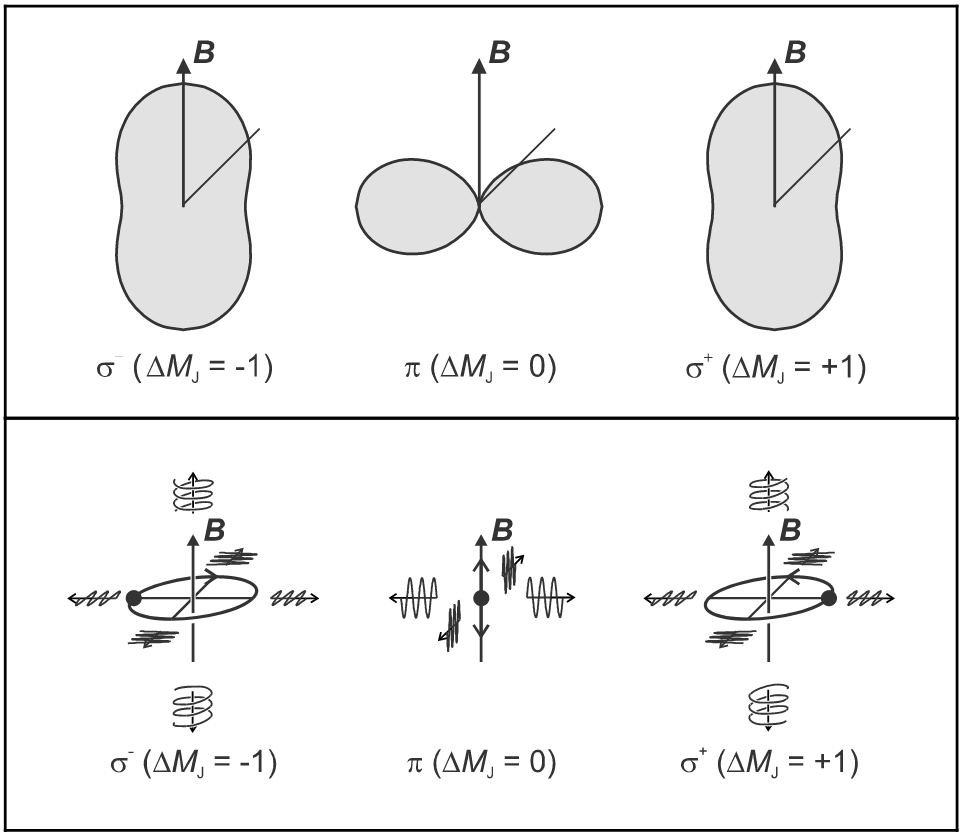
\includegraphics[width=.8\linewidth]{zeeman-abstrahlung}
  \caption{Polarisationsverteilung und Abstrahlungscharakteristik elektrischer Dipolübergänge \cite{Anleitung} \cite{Leybold}.}
  \label{fig:zeeman-abstrahlung}
\end{figure}

Das am Okular enstehende Bild ist in Abb. \ref{fig:zeeman-transveral-ohne-ohne} gezeigt.
\begin{figure}[H]
  \centering
  % 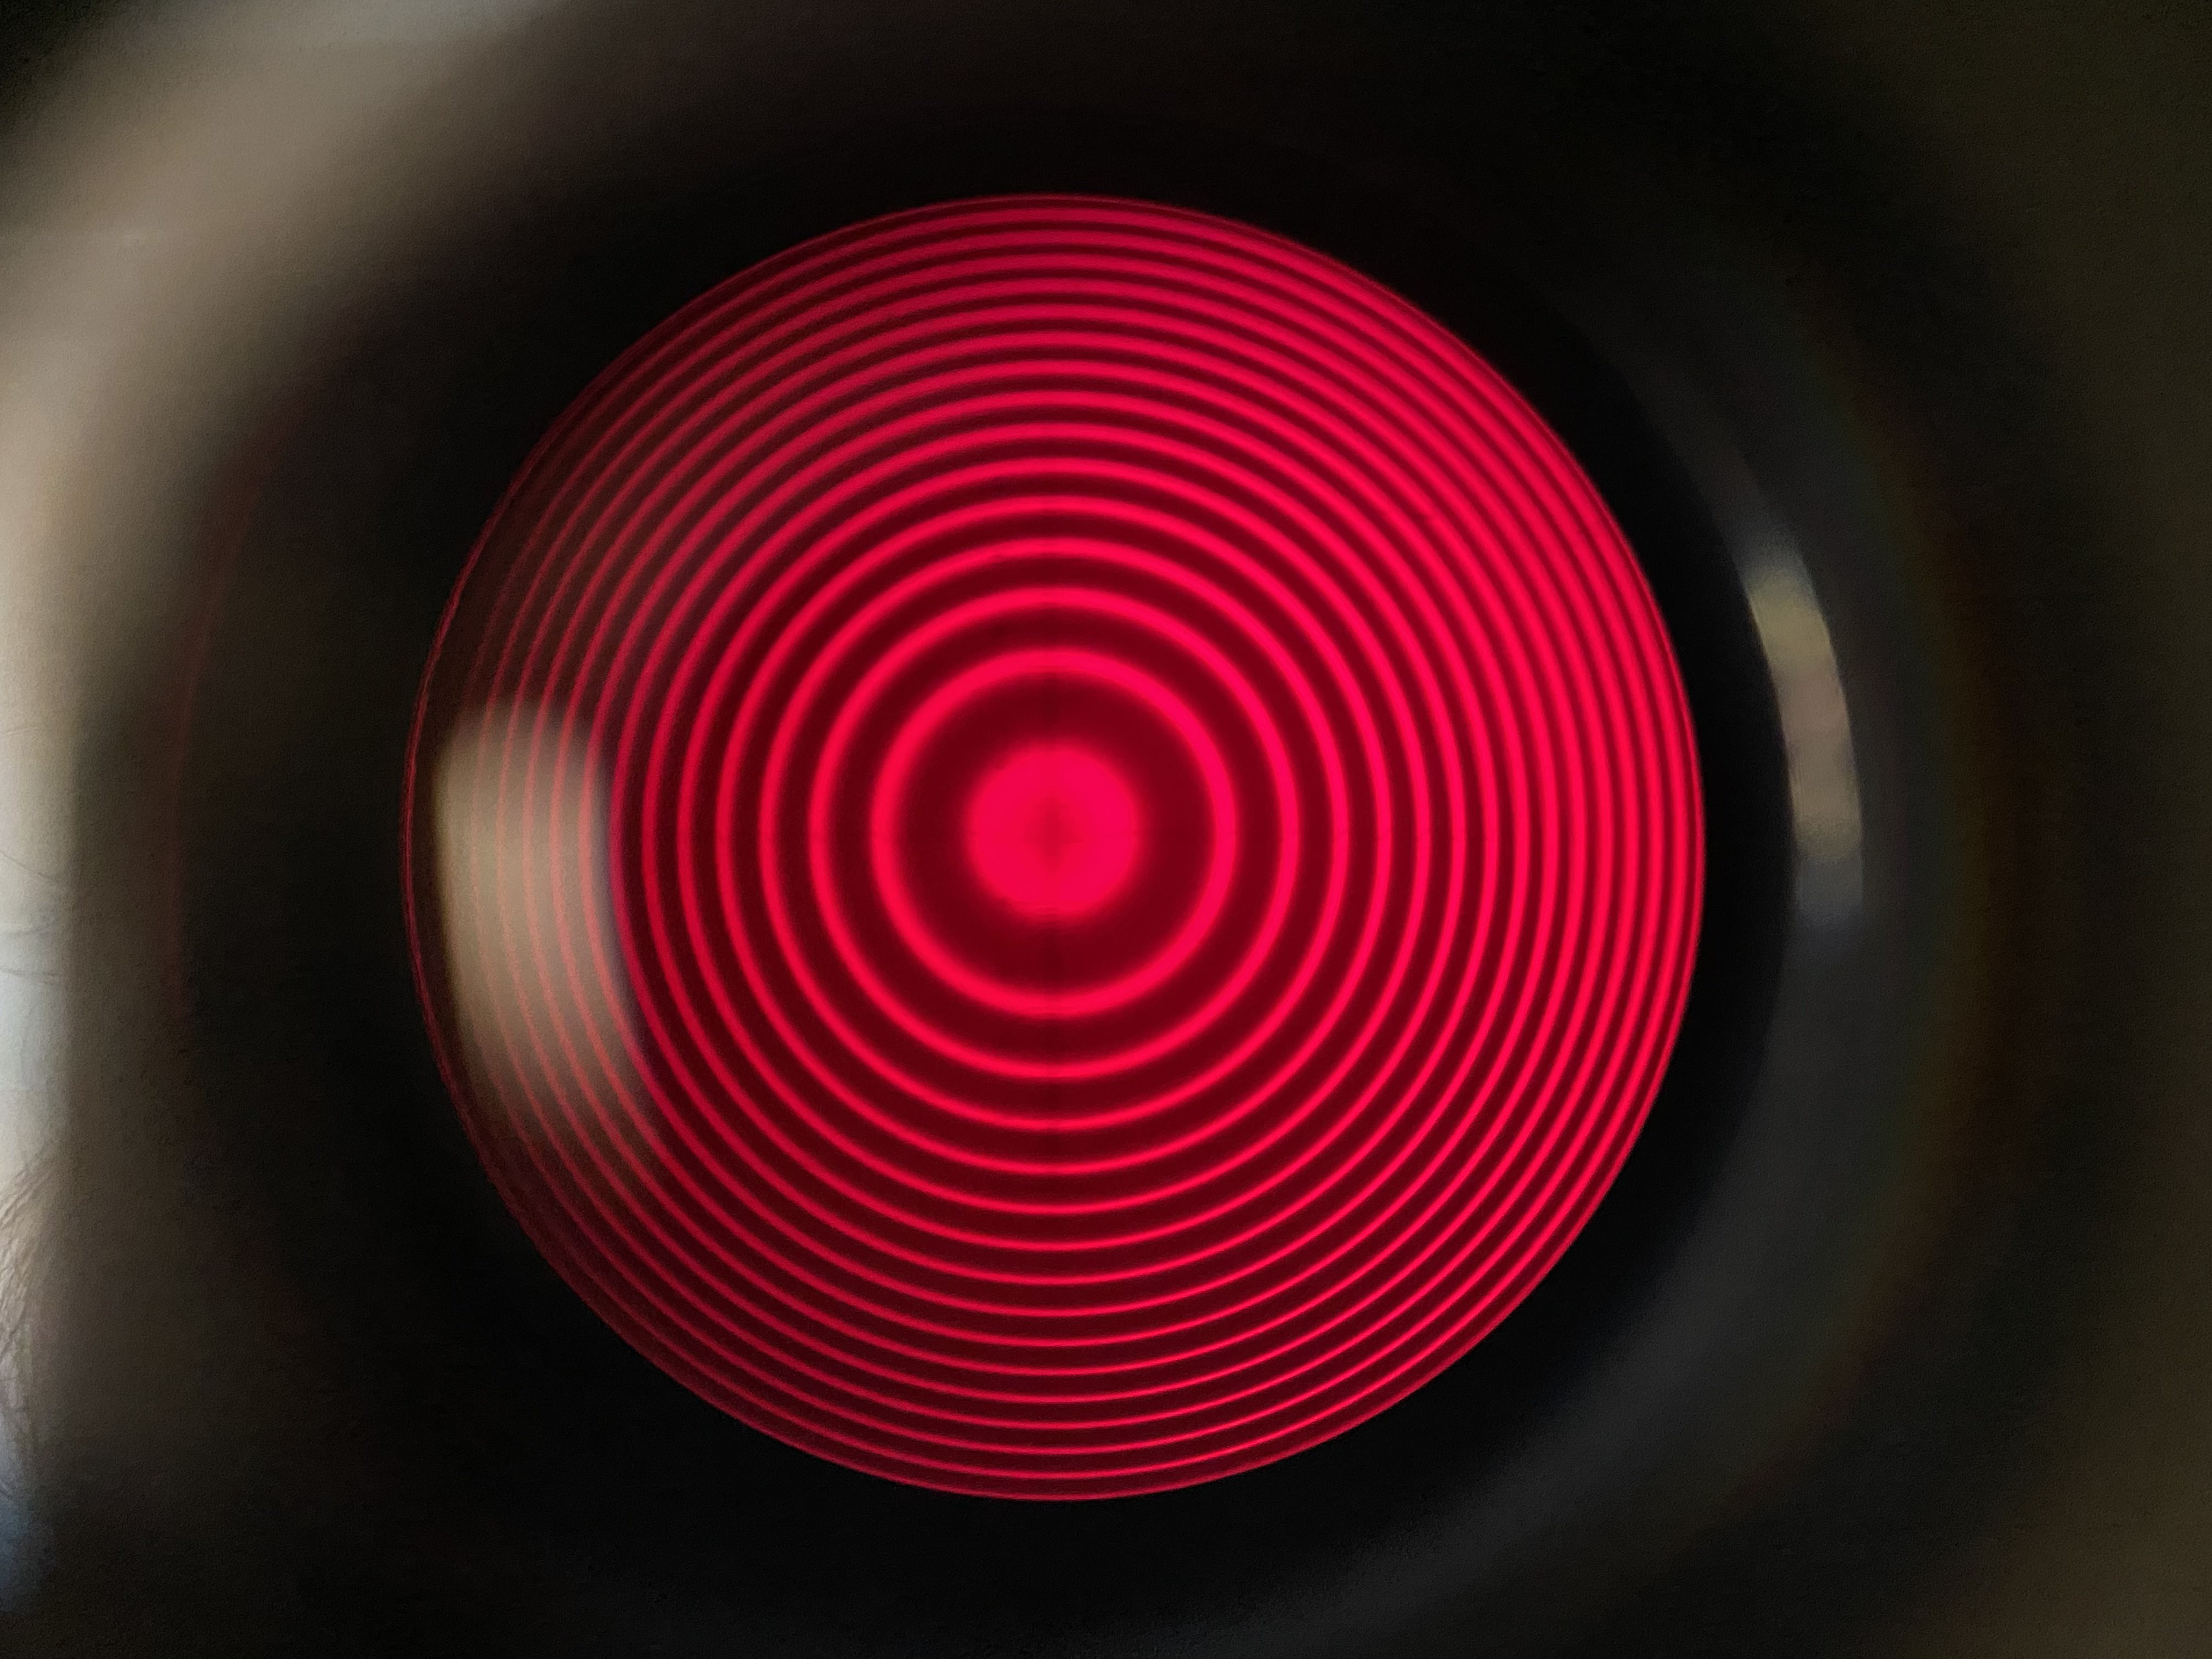
\includegraphics[width=.8\linewidth]{zeeman-transversal-ohne-ohne}
  \caption{Interferenzmuster bei transversaler Beobachtung ohne Magnetfeld, ohne Polarisationsfilter.}
  \label{fig:zeeman-transveral-ohne-ohne}
\end{figure}
Es sind die verschiedenen Interferenzringe zu erkennen, die hier alle von der gleichen Wellenlänge stammen.

Nun wird das Magnetfeld eingeschaltet und erhöht, bis man eine Aufspaltung der Ringe sieht, siehe Abb. \ref{fig:zeeman-transveral-mit-ohne}
\begin{figure}[H]
  \centering
  % 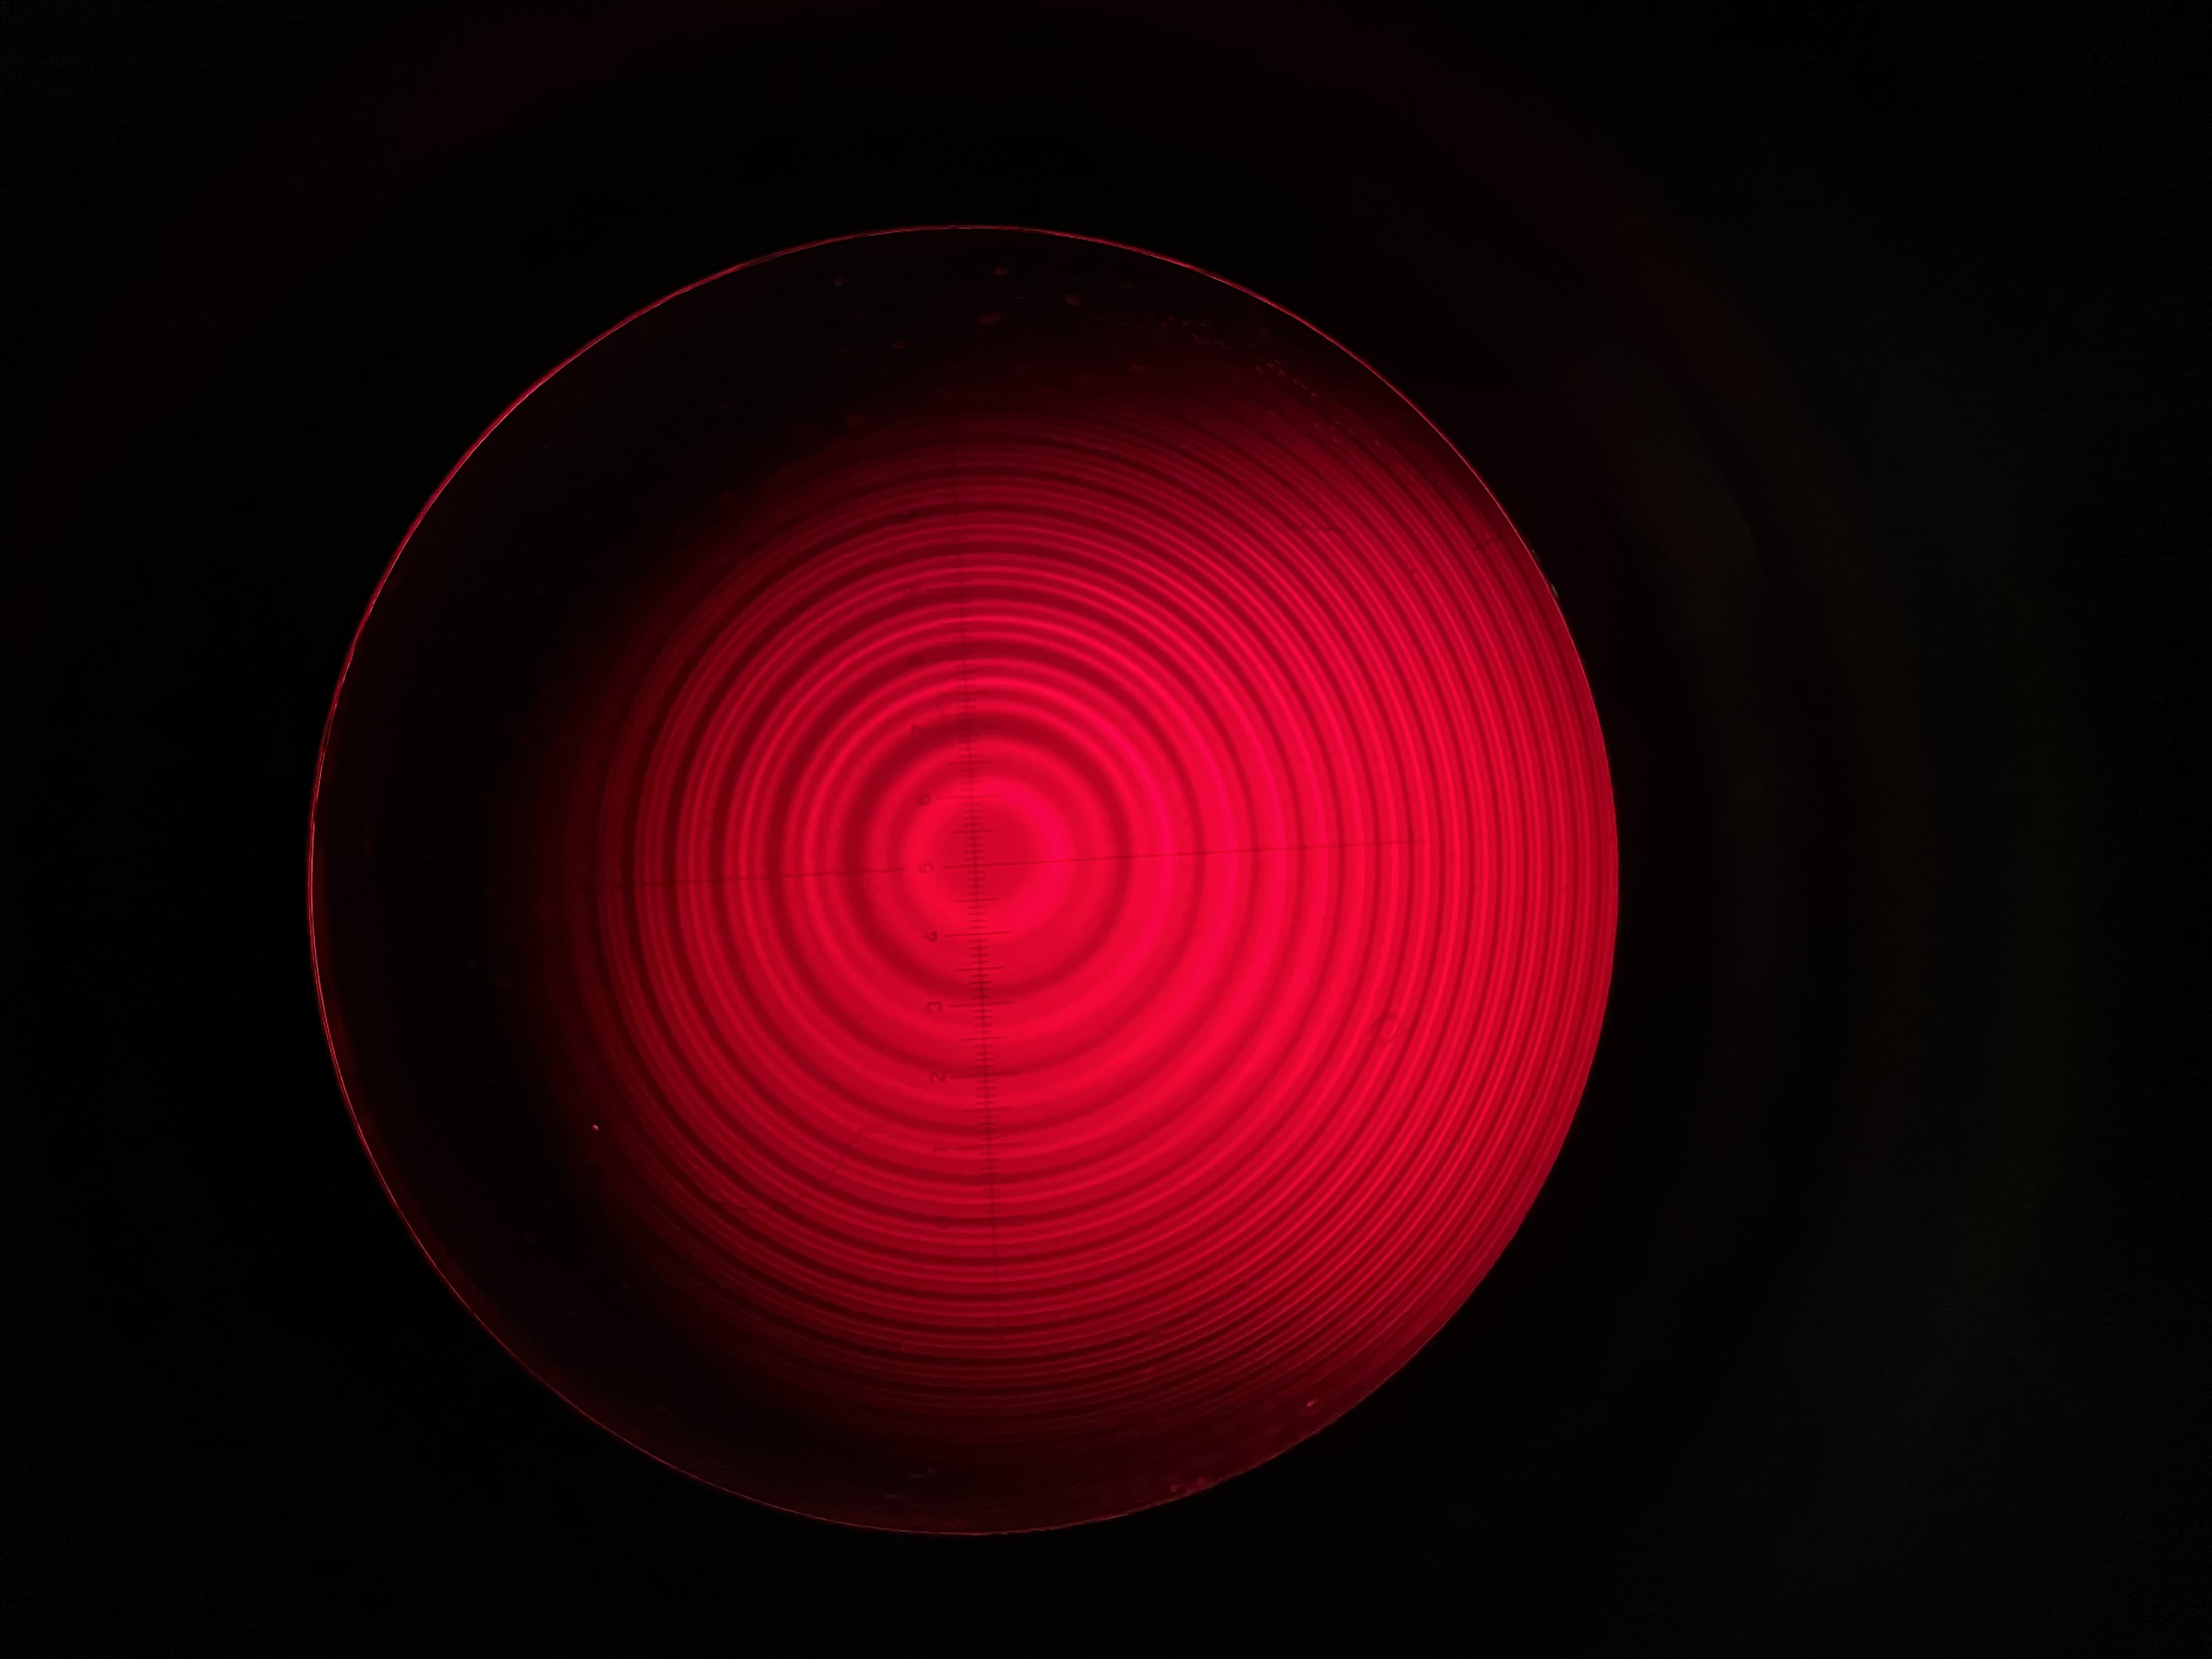
\includegraphics[width=.8\linewidth]{zeeman-transversal-mit-ohne}
  \caption{Interferenzmuster bei transversaler Beobachtung mit Magnetfeld, ohne Polarisationsfilter.}
  \label{fig:zeeman-transveral-mit-ohne}
\end{figure}
Durch den Zeeman-Effekt gibt es eine Energieaufspaltung $\Delta E \propto B_zM_J$ der Niveaus.
Dadurch sind die $\pi$-Übergänge unbeeinflusst, während die $\sigma^+$- bzw. $\sigma^-$-Übergänge
eine etwas geringere bzw. höhere Wellenlänge produzieren. Was zuvor ein Ring war, spaltet sich daher in drei Ringe auf.

Die verschiedenen Komponenten können durch Einsatz des Polarisationsfilters herausgefiltert werden (Abb. \ref{fig:zeeman-transveral-mit-90}, \ref{fig:zeeman-transveral-mit-0}).
\begin{figure}[H]
  \centering
  % 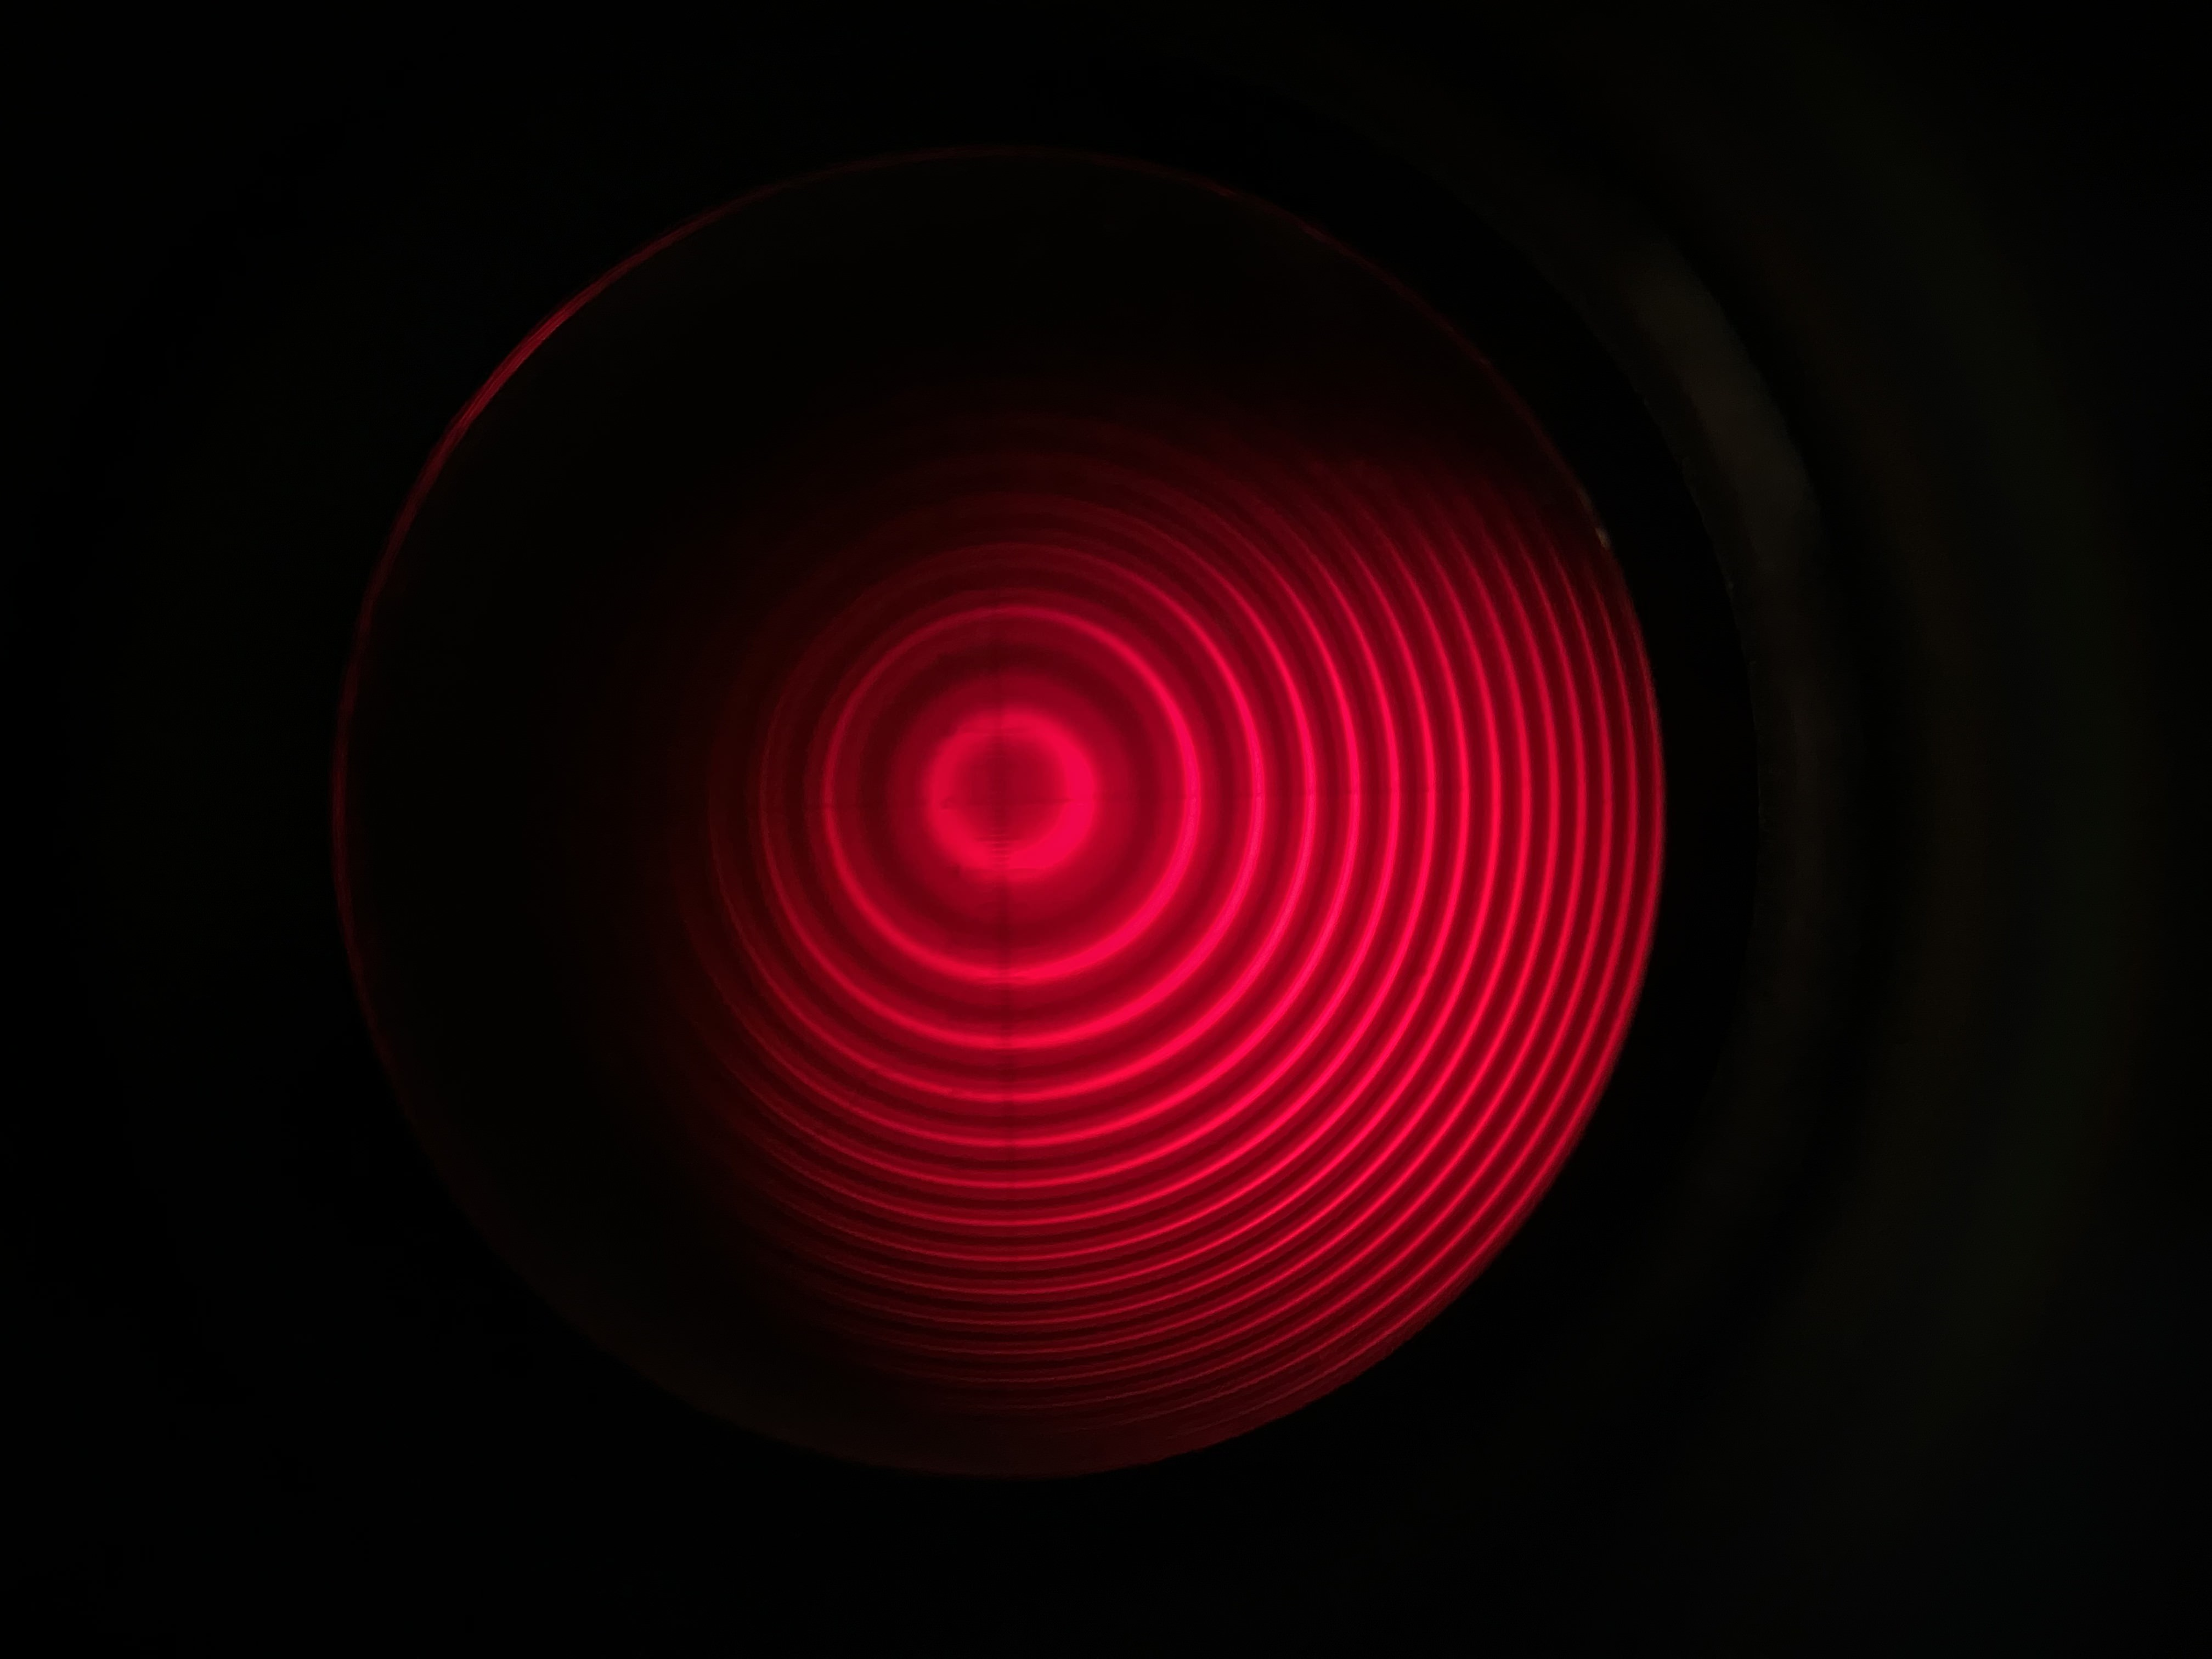
\includegraphics[width=.8\linewidth]{zeeman-transversal-mit-90}
  \caption{Interferenzmuster bei transversaler Beobachtung mit Magnetfeld, mit Polarisationsfilter auf \ang{90}.}
  \label{fig:zeeman-transveral-mit-90}
\end{figure}
\begin{figure}[H]
  \centering
  % 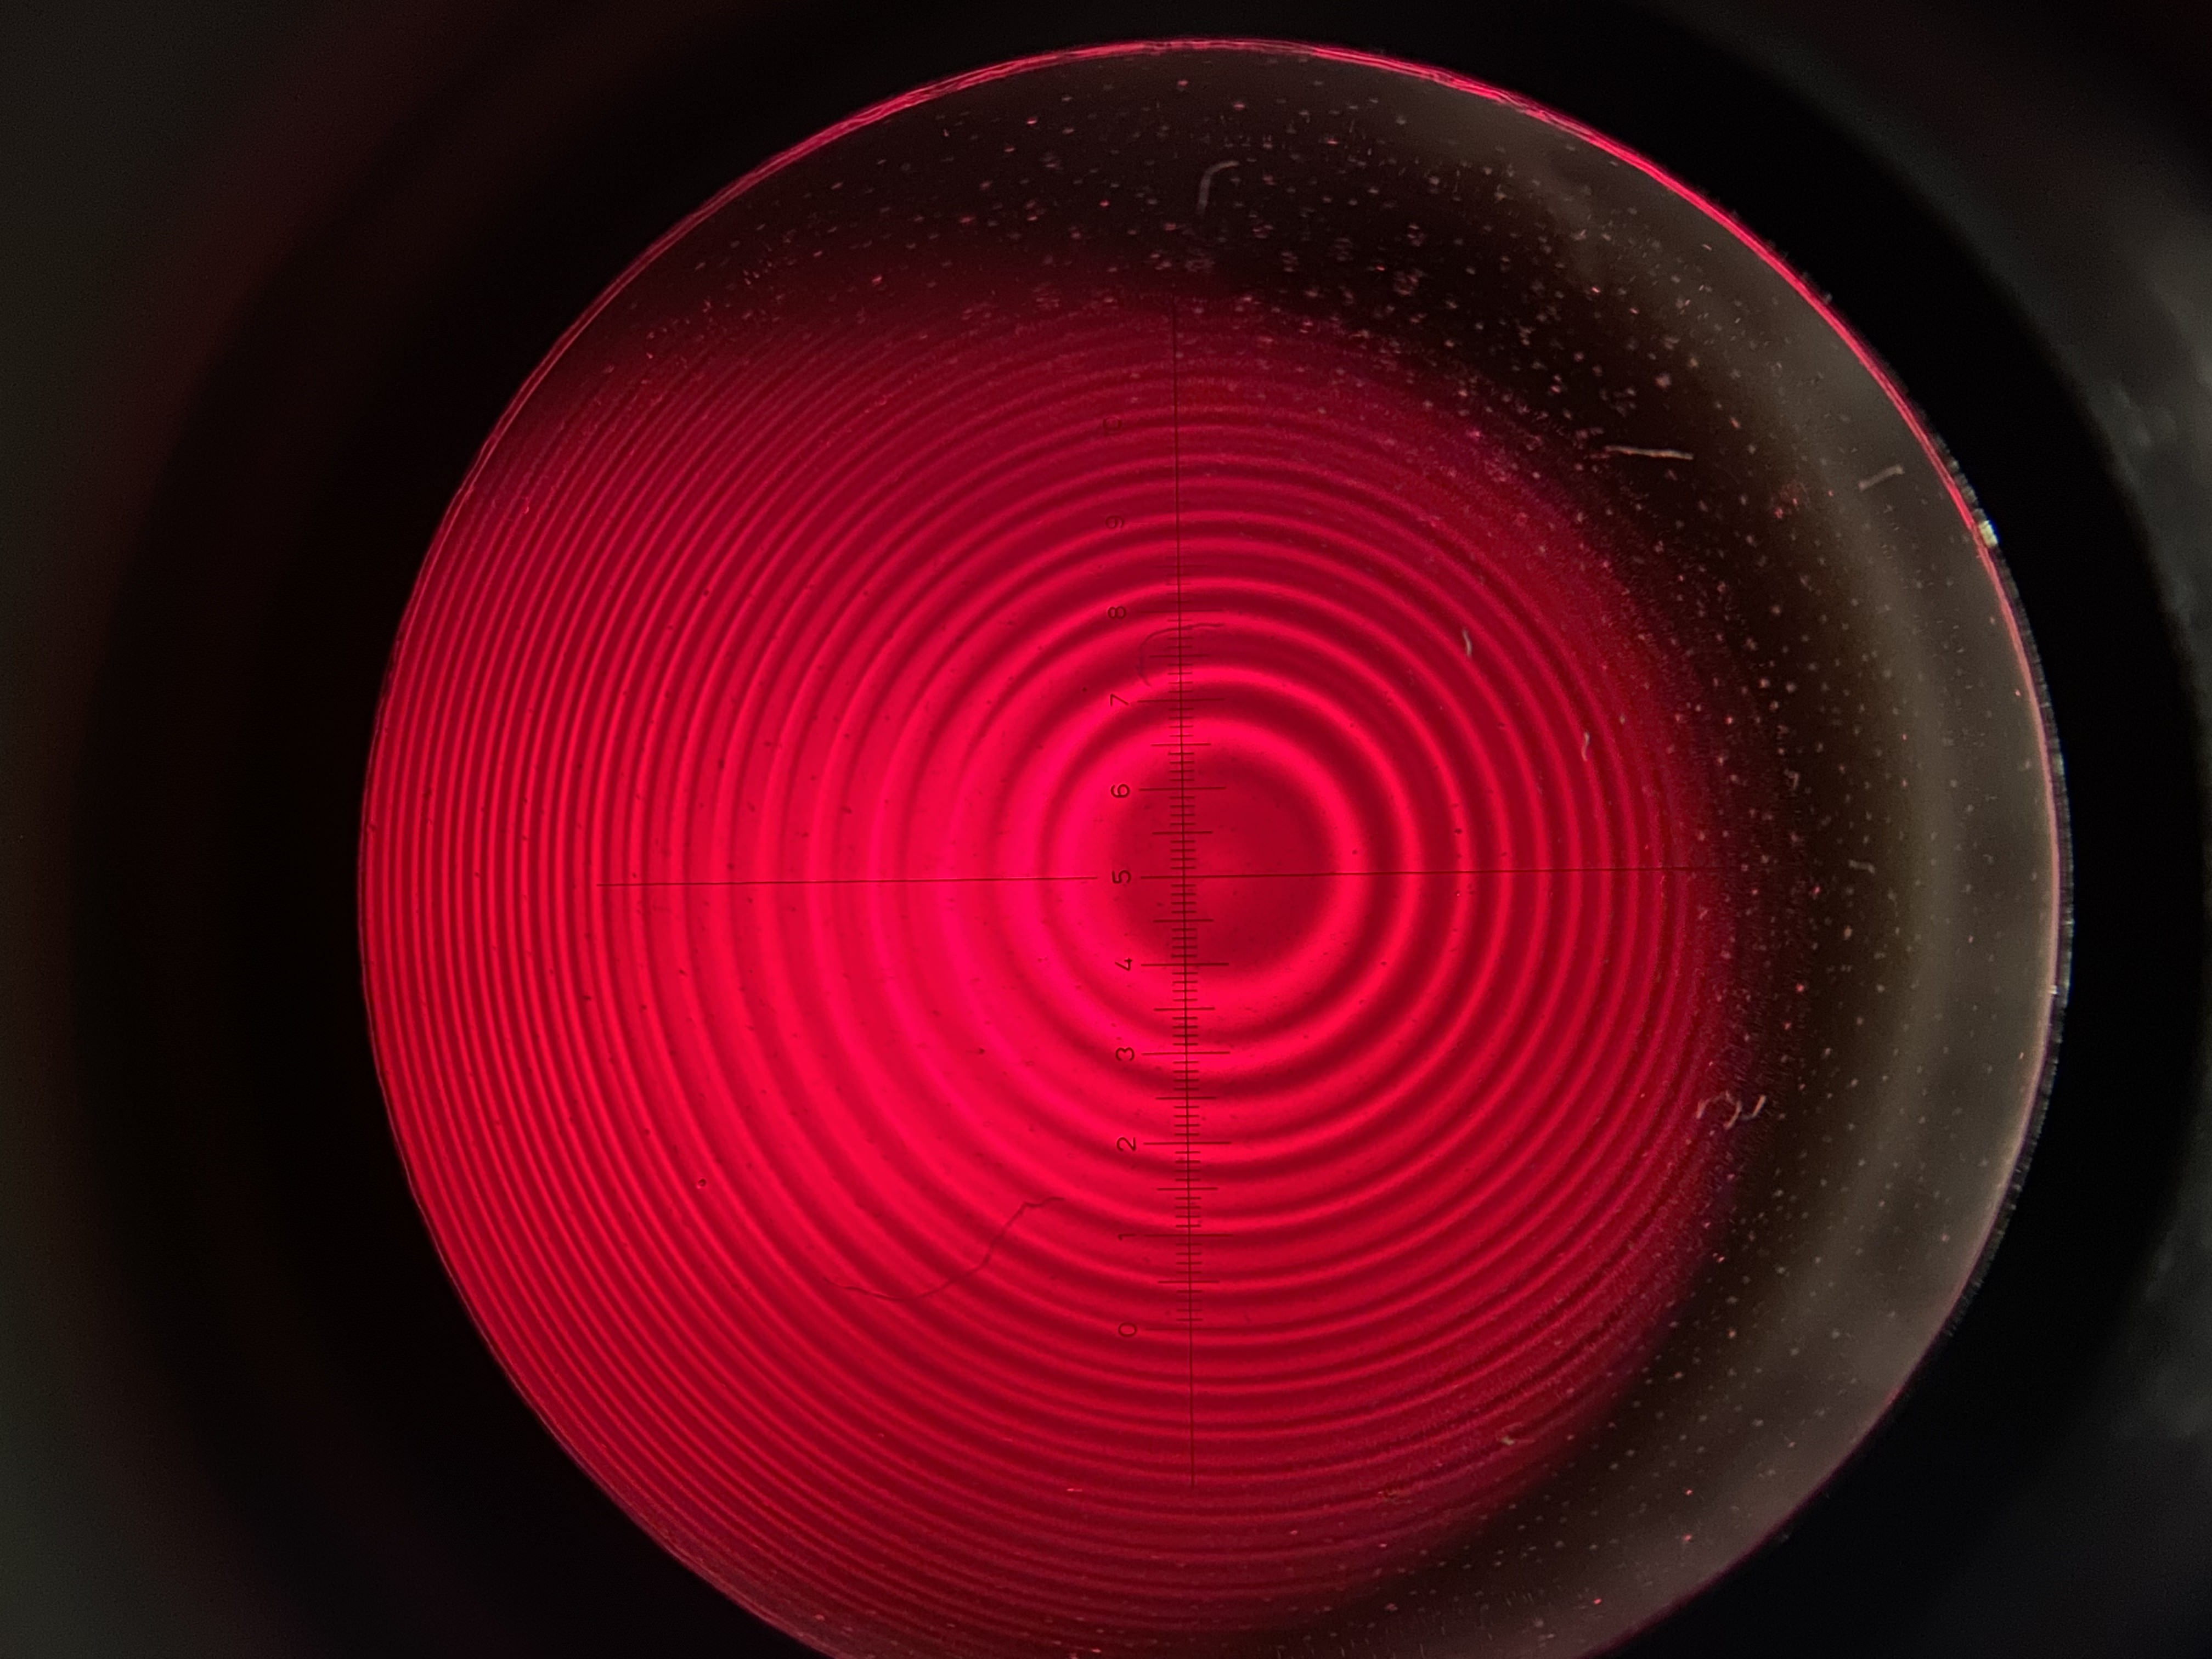
\includegraphics[width=.8\linewidth]{zeeman-transversal-mit-0}
  \caption{Interferenzmuster bei transversaler Beobachtung mit Magnetfeld, mit Polarisationsfilter auf \ang{0}.}
  \label{fig:zeeman-transveral-mit-0}
\end{figure}
Wenn der Filter auf \ang{90} steht, sind wieder nur einzelne Ringe zu sehen, die dem $\pi$-Übergang entsprechen,
welche Licht mit Polarisation parallel zum Magnetfeld produziert.
Steht der Filter auf \ang{0}, gibt es jeweils zwei Ringe, die $\sigma^+$ bzw. $\sigma^-$ entsprechen.

\todo{Auflösungsvermögen}

\subsubsection{longitudinale Konfiguration}
Die Magneten mitsamt der Cadmiumlampe werden um \ang{90} gedreht,
um die Beobachtungen in longitudinaler Konfiguration (Magnetfeld parallel zur optischen Achse bzw. der Beobachtungsrichtung)
zu wiederholen.

Ohne Magnetfeld ergibt sich das Muster in Abb. \ref{fig:zeeman-longitudinal-ohne-ohne}, was mit der entsprechenden Beobachtung
bei transversaler Konfiguration übereinstimmt.
\begin{figure}[H]
  \centering
  % 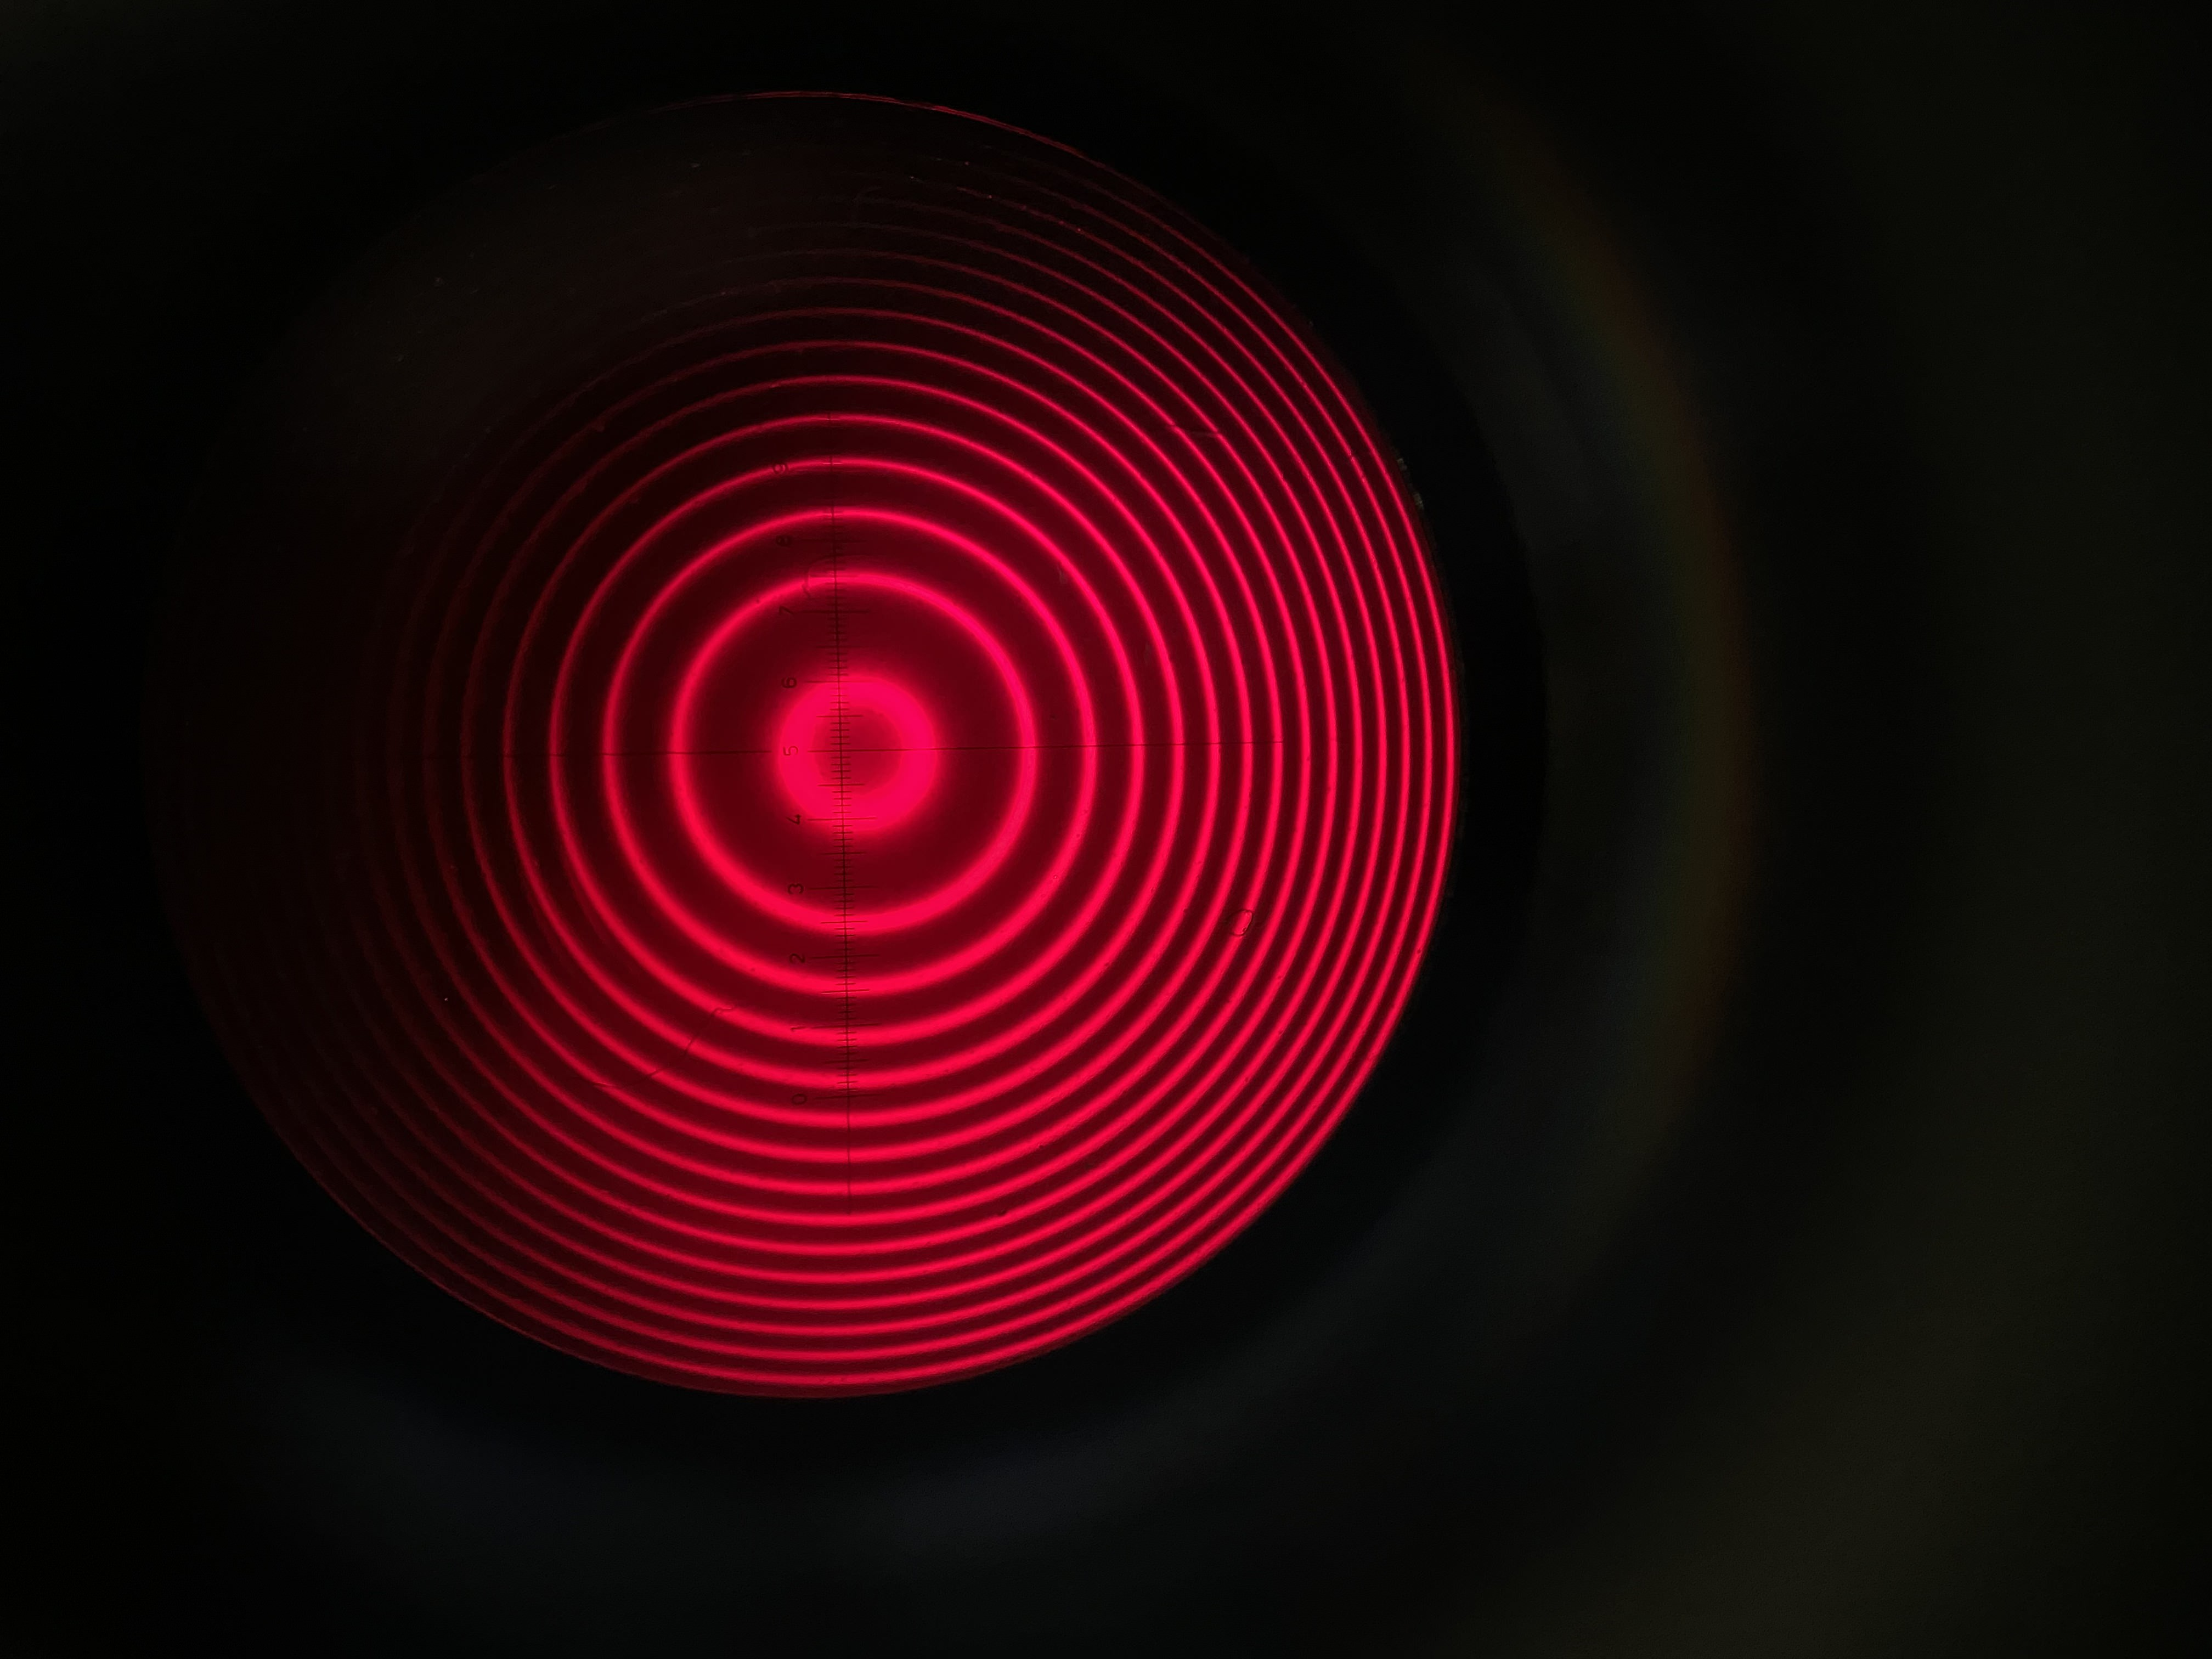
\includegraphics[width=.8\linewidth]{zeeman-longitudinal-ohne-ohne}
  \caption{Interferenzmuster bei longitudinaler Beobachtung ohne Magnetfeld, ohne Polarisationsfilter.}
  \label{fig:zeeman-longitudinal-ohne-ohne}
\end{figure}

Wird das Magnetfeld angeschaltet (Abb. \ref{fig:zeeman-longitudinal-mit-ohne}), ist eine Aufspaltung in jeweils zwei Ringe zu beobachten.
Diese entsprechen den beiden $\sigma$-Übergängen, während der $\pi$-Übergang aufgrund seiner Abstrahlungscharakteristik
in longitudinaler Konfiguration nicht zu sehen ist.
\begin{figure}[H]
  \centering
  % 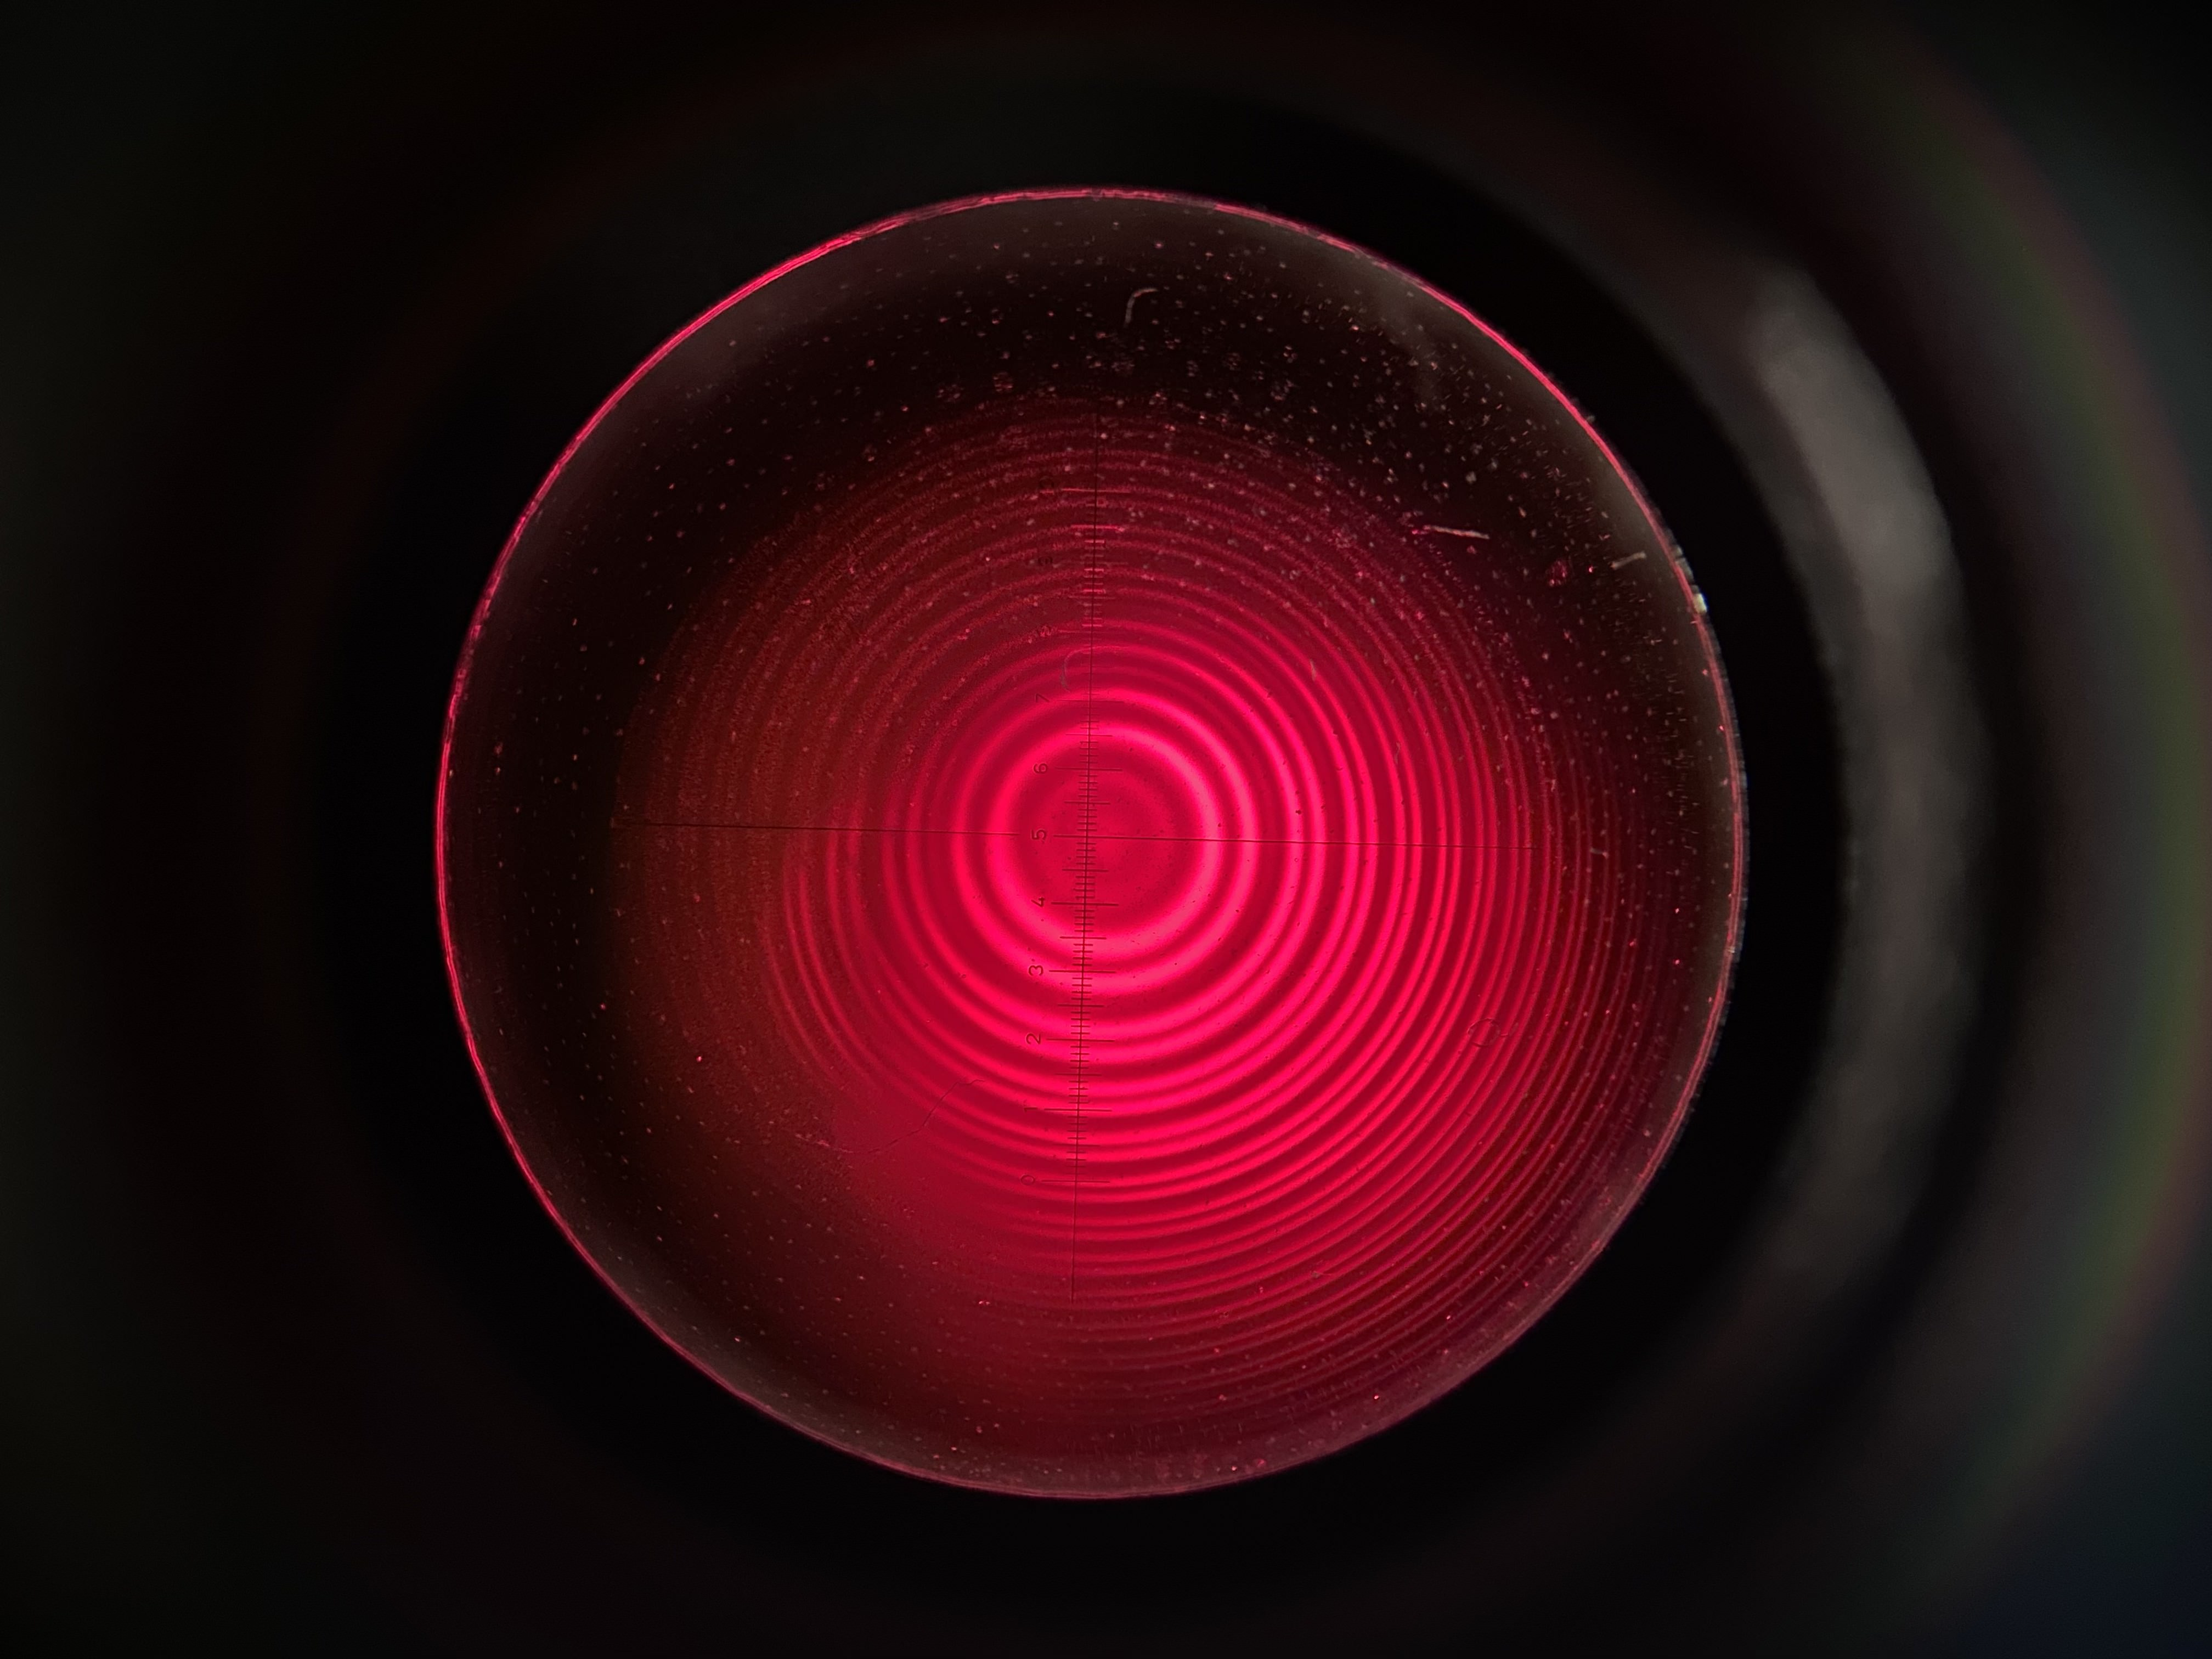
\includegraphics[width=.8\linewidth]{zeeman-longitudinal-mit-ohne}
  \caption{Interferenzmuster bei longitudinaler Beobachtung mit Magnetfeld, ohne Polarisationsfilter.}
  \label{fig:zeeman-longitudinal-mit-ohne}
\end{figure}

Als nächstes wird zusätzlich eine $\lambda / 4$-Platte in \ang{0}-Stellung in den Strahlengang vor dem
Polarisationsfilter eingesetzt. Diese dient dazu, das rechts- bzw. linkspolarisierte Licht der $\sigma$-Übergänge
(siehe Abb. \ref{fig:zeeman-abstrahlung}) zu verschiedenen linearen Polarisationsrichtungen umzuwandeln,
welche dann mit dem Polarisationsfilter ausgewählt werden können.

Mit dem Polarisationsfilter auf \ang{-45} ist nur noch jeweils ein Ring stark zu sehen (Abb. \ref{fig:zeeman-longitudinal-mit--45})
\begin{figure}[H]
  \centering
  % 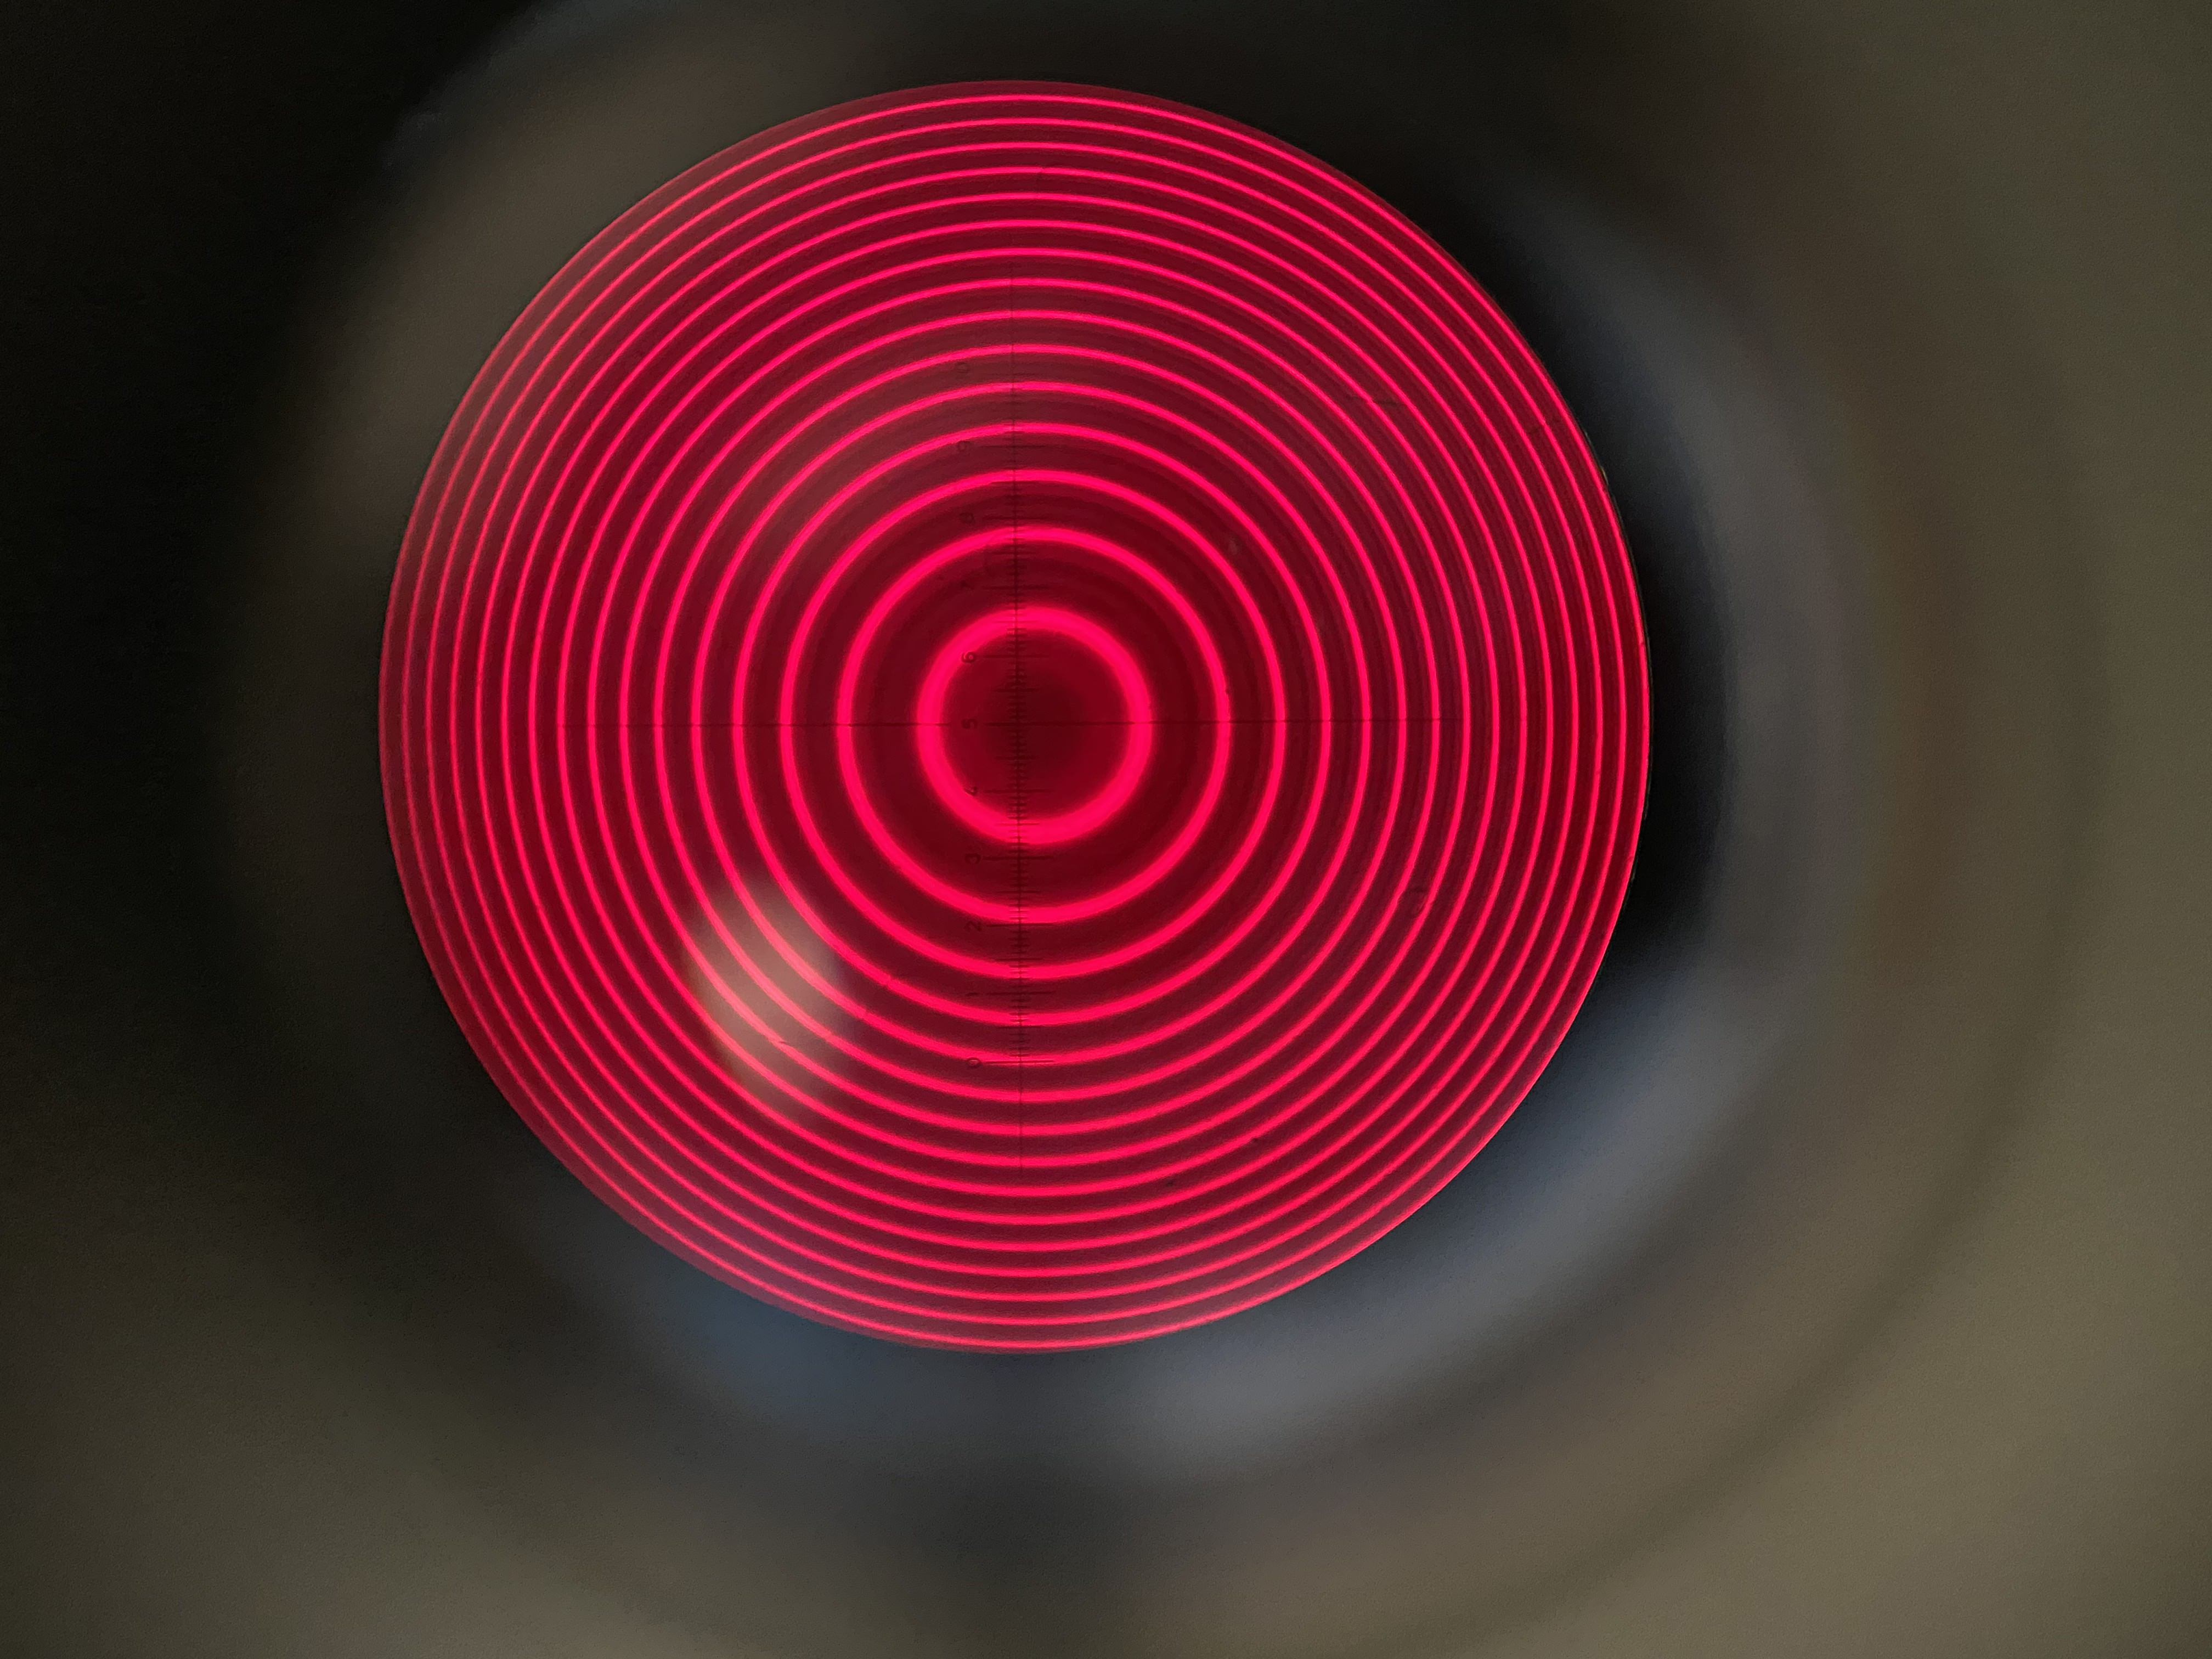
\includegraphics[width=.8\linewidth]{zeeman-longitudinal-mit--45}
  \caption{Interferenzmuster bei longitudinaler Beobachtung mit Magnetfeld, mit Polarisationsfilter.}
  \label{fig:zeeman-longitudinal-mit--45}
\end{figure}

Mit dem Polarisationsfilter in \ang{45}-Stellung ist nur der jeweils andere Ring stark zu sehen (Abb. \ref{fig:zeeman-longitudinal-mit-45}).
\begin{figure}[H]
  \centering
  % 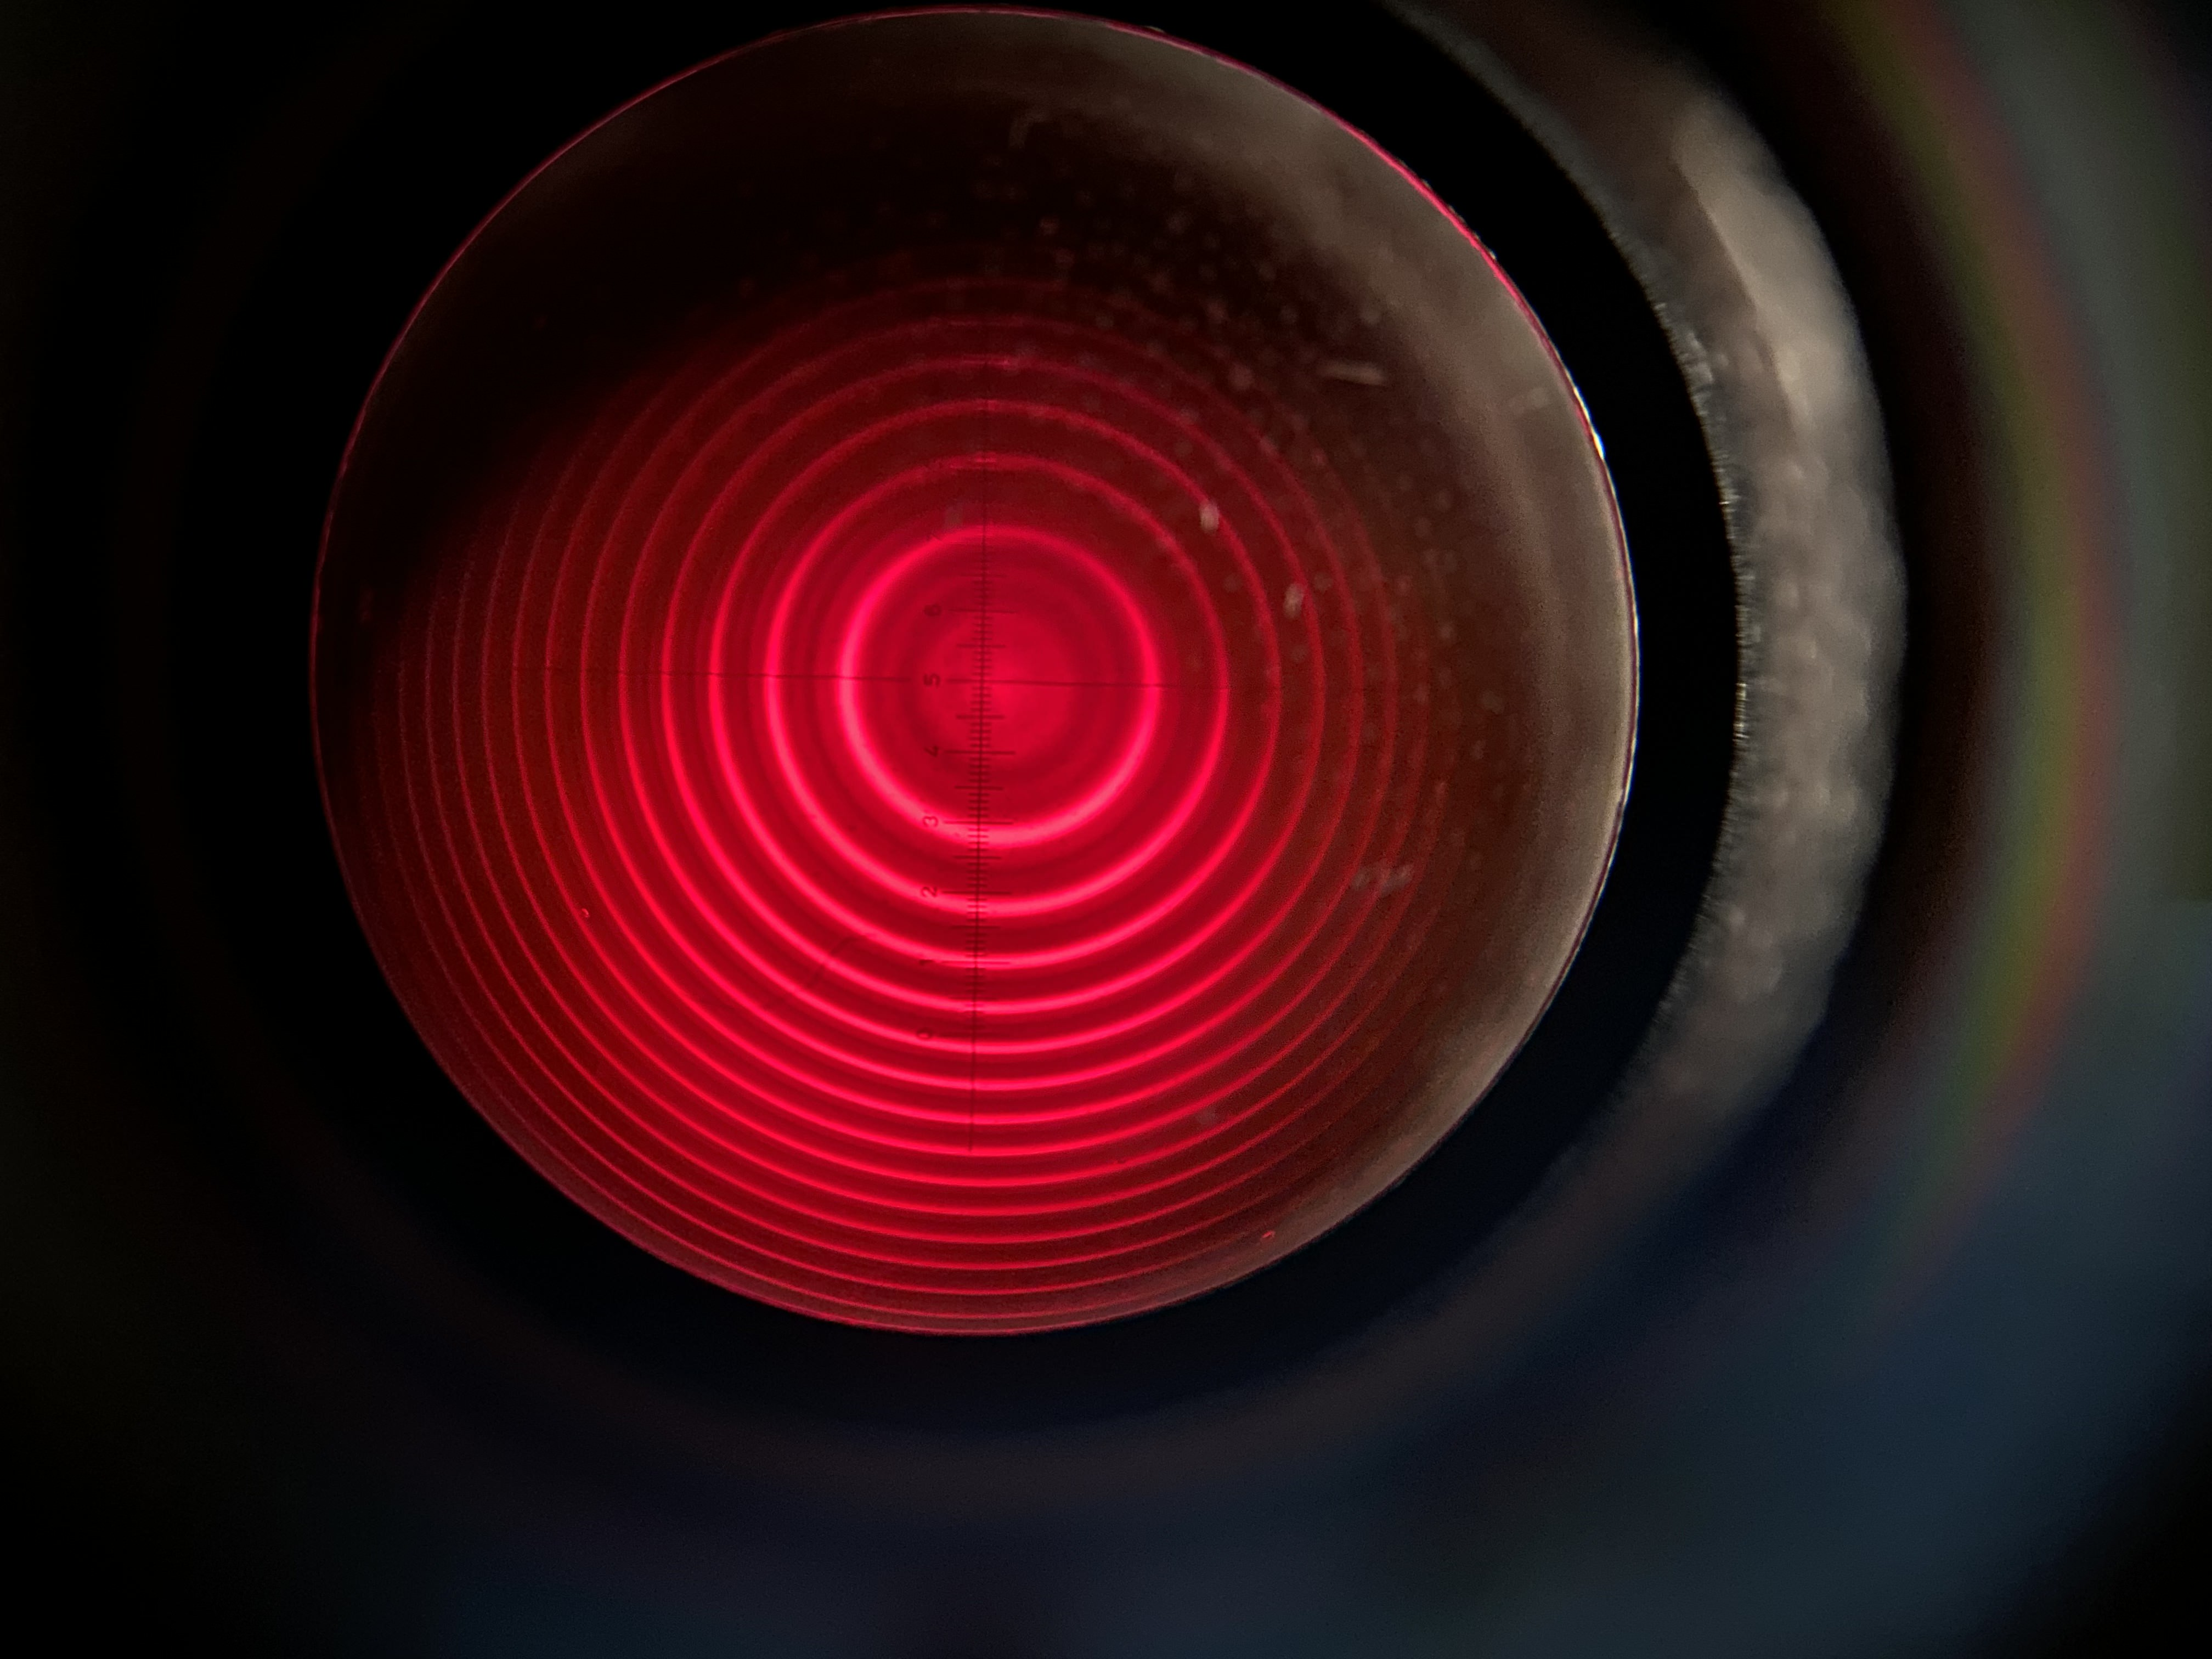
\includegraphics[width=.8\linewidth]{zeeman-longitudinal-mit-45}
  \caption{Interferenzmuster bei longitudinaler Beobachtung mit Magnetfeld, mit Polarisationsfilter.}
  \label{fig:zeeman-longitudinal-mit-45}
\end{figure}


\subsection{Messung des Zeeman-Effekts}
Es soll nun quantitativ die Stärke der Aufspaltung in Abhängigkeit des anliegenden Magnetfelds gemessen werden.
Hierzu wird die transversale Konfiguration verwendet.

\subsubsection{Magnetfeldkalibrierung}
Es wird die Abhängigkeit der Magnetfeldstärke vom fließenden Strom durchmessen, um daraus eine Kalibrierungskurve zu erstellen.
Hierzu wird anstatt der Cadmiumlampe eine Hall-Sonde genau mittig zwischen den Polschuhen eingeführt.
In Reihe zu den Magneten wird ein \enquote{Cassy-Modul} eingeschaltet,
wodurch am Computer mithilfe einer speziellen Software die Abhängigkeit automatisch aufgezeichnet werden kann.
Die Messung wird gestartet und der Strom allmählich bis zum maximal erreichbaren Wert hochgefahren.
Dann wird die Messung gestoppt und der Strom wieder ausgeschaltet.

In Abb. \ref{} sind die Messdaten zusammen mit einem $\Chi^2$-Fit der Form
\[
  B(I) = a + bI + cI^2
\]
dargestellt. Als Fehlerwerte auf $I$ und $B$ wurden dabei $2\%$ des jeweiligen Werts angesetzt,
wobei Fehlerwerte von $\SI{0.002}{\A}$ und $\SI{0.2}{\mT}$ nicht unterschritten werden dürfen.



\clearpage
\section{Fazit}


\clearpage
\begin{thebibliography}{9}

\bibitem{Anleitung}
\textit{Physikalisches Praktikum Teil IV -- Versuchsbeschreibungen}, Universität Bonn, Abruf 29.10.2024

\bibitem{Leybold}
\textit{Beobachtung des normalen Zeeman-Effekts in transversaler und longitudinaler Konfiguration}, Leybold Didactic, Abruf 30.10.2024

\end{thebibliography}

\end{multicols}

\end{document}

